\chapter{Implémentation}
\section{Projet Android}
Un projet Android est découpé selon une arborescence précise.
Lors de la création d'un projet, sous Eclipse, il faut choisir le nom du projet.
Ce projet appartient à un package qui se présente sous la forme suivante :
"extension\_domaine"."nom\_de\_domaine".android."nom\_du\_projet". Il faut
ensuite choisir le nom de l'Activity qui sera lancée au démarrage. Pour
finir, il faut choisir le nom de l'application qui sera affiché dans le menu principal.
Aprés la création du projet, nous obtenons une architecture prédéfinie, qui
contient plusieurs dossiers et fichiers:
\begin{itemize}
  \item Un dossier \textit{src} qui devra contenir l'ensemble des fichiers
  sources d'un même package (plusieurs packages peuvent être créés dans le
  dossier \textit{src})
  \item Un fichier \textit{R.java}, généré par l'ADT, qui contient l'ensemble
  des références aux ressources du projet
  \item Un dossier \textit{assets}, qui contient l'ensemble des données qui
  seront chargées sur le mobile (ou tablette) lors de la compilation
  \item Un dossier \textit{res}, qui contient l'ensemble des ressources
  relatives aux projet. Ce dossier contient plusieurs sous-dossiers:
  \begin{itemize}
    \item Le dossier \textit{drawable} contient l'ensemble des images utilisées
    par l'application
    \item Le dossier \textit{layout} contient les fichiers \textit{.xml} qui
    décrivent les interface de l'application
    \item Le dossier \textit{values} contient des fichiers qui décrivent les
    constantes utilisées par l'application
    \item Le dossier \textit{menu} contient les differents menus utilisés
    \item Le dossier \textit{xml} contient le ficher de mise en forme du
    \textit{SharedPreferences} utilisé
    \item Les dossiers \textit{values-[CodeLangue]} contiennent les traductions
    des chaînes utilisées dans le projet.
   \end{itemize}
   \item Pour conclure, nous trouvons un fichier
   \textit{AndroidManifest.xml} qui définit le comportement de l'application.
   Nous y trouvons par exemple le nom, l'icône par défaut, le thème, la version
   minimale, les activités, les services de l'application, etc\ldots
\end{itemize}
\section{L'objet Caméra}
\subsection{Description}
L'objet Caméra est implémenté dans la classe \textit{Camera.java}.\newline
Celle-ci regroupe les informations suivantes : 
\begin{itemize} 
\item un descriptif de la caméra. Exemple : ``Caméra du Jardin''
\item le protocole de communication à utiliser (HTTP ou RTSP).
\item l'URL d'accès. Exemple : ``http://192.168.1.20''
\item le port (par défaut le port 80 est utilisé).
\item le nom d'utilisateur (login).
\item le mot de passe.
\item le canal (nécessaire lors de l'utilisation de plusieurs caméras pour une
même adresse).
\item un identifiant unique appelé \textit{uniqueID} défini par la position de
la caméra dans la liste sur la page d'accueil.
\item le groupe assigné lors de la mise en route de la détection de mouvements
(compris entre 0 et 9) appelé \textit{groupeID}.\\
\end{itemize}
\indent Afin de pouvoir communiquer une caméra entre plusieurs \textit{activités
(activity)} nous avons choisi de rendre cette classe \textit{serializable} pour
ne pas devoir passer une à une chacune des caractéristiques.\\
Cette classe contient également une primitive capable de générer un entier
unique pour le couple \textit{uniqueID} et \textit{groupID}, afin de pouvoir
lancer plusieurs fenêtres de détection de mouvements pour une même caméra
(\textit{getMotionDetectionID}).
\subsection{Construction de l'objet}
La création d'une caméra se fait via l'interface graphique définie par le
fichier \textit{add\_cam.xml}.\newline

Nous y retrouvons des champs de texte éditables pour chacune
des caractéristiques de la caméra ainsi qu'un bouton permettant l'ajout de caméra via \textit{QRCode}.\newline
Un \textbf{QRCode} est un code-barres à deux dimensions. Selon
\textit{Wikipedia}\footnote{\label{zxing}http://fr.wikipedia.org/wiki/Code\_QR}
un QRCode peut contenir plus de 4296 caractères alphanumériques contre 10 à 13
pour un code-barre classique.\newline
L'exemple suivant illustre l'équivalence \textit{caméra-représentation
xml-QRCode}\newline
\begin{figure}[H]
  \centering
  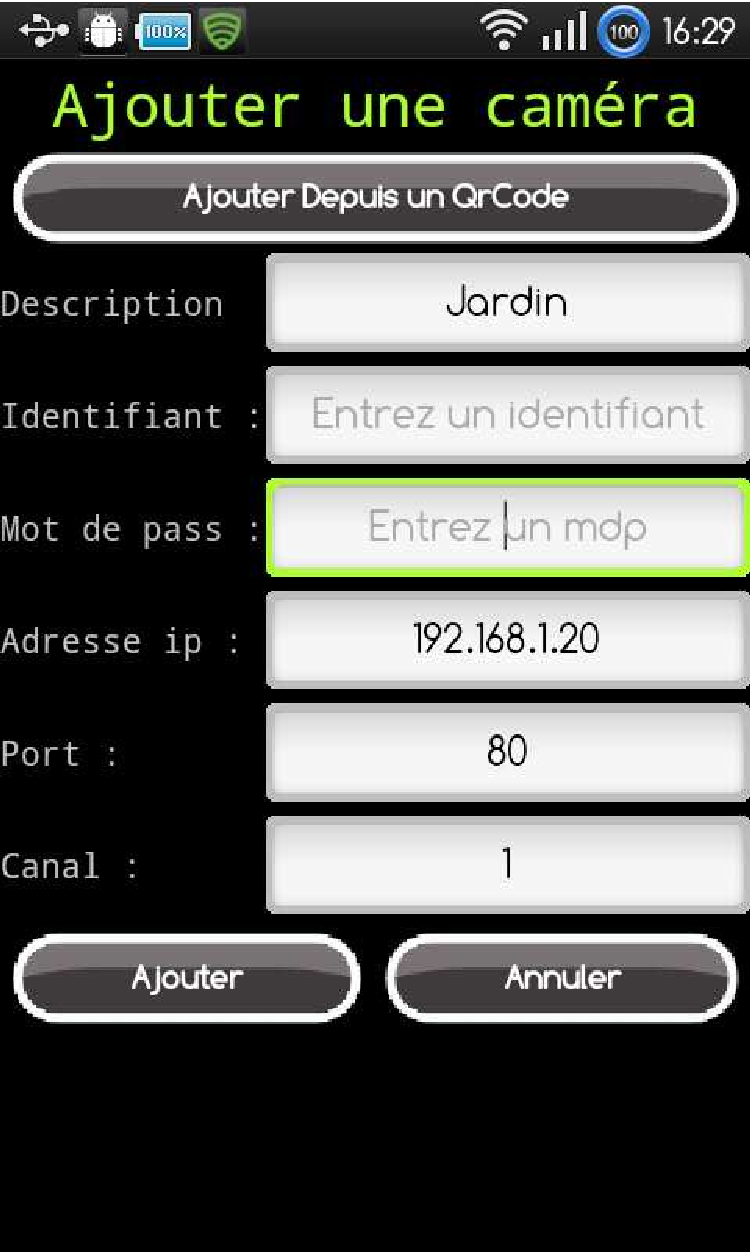
\includegraphics[scale=0.4]{Images/addCam.pdf}
  
\includegraphics{Images/chart.pdf}
  \begin{lstlisting}[format=XML]
<?xml version='1.0' encoding='UTF-8' standalone='yes'?>
<camList>
<camera>
<id>Jardin</id>
<adresse>http://192.168.1.20:80</adresse>
<channel>1</channel>
</camera>
</camList>
\end{lstlisting}
\end{figure}

\indent Le lecteur de codes QR est implémenté par la bibliothèque
\textit{zxing}\footnote{\label{zxing} http://code.google.com/p/zxing/}. 
Lors d'un clic sur ce bouton, nous appelons l'activité 
\textit{SCAN} de la bibliothèque zxing avec comme argument
\textit{QR\_CODE\_MODE}.
Si la bibliothèque n'est pas disponible sur l'appareil, nous faisons appel à
\textit{l'Android market} afin de télecharger l'application \textit{zxing} (qui
implémente l'ensemble des fonctions proposées par la bibliothèque).
\newline
\begin{lstlisting}[caption={Lancement de l'activité zxing ou de l'Android
market.}] 
    public void onClick(View v) { try {
            Intent intent = new Intent(
                "com.google.zxing.client.android.SCAN");
            intent.putExtra("SCAN_MODE", "QR_CODE_MODE");
            startActivityForResult(intent, 0);
        } catch (ActivityNotFoundException e) {
            String marketSearch = "market://details?id=com.google.zxing.client.android";
            Intent updateIntent = new Intent(Intent.ACTION_VIEW, Uri.parse(marketSearch));
            startActivity(updateIntent);
        }
    }
\end{lstlisting}

\indent \newline
\indent Il existe plusieurs générateurs de codes QR disponibles sur internet
dont celui implémenté par la bibliothèque
\textit{zxing}\footnote{\label{zxingGenerator}
http://zxing.appspot.com/generator/}.

\indent Pour ajouter la nouvelle
caméra, il ne reste à l'utilisateur qu'à cliquer sur le bouton
\textit{Ajouter} pour revenir sur l'écran d'accueil et constater l'ajout de la
caméra. Cependant il reste possible de revenir à l'écran d'accueil sans
sauvegarder les changements en cliquant sur \textit{Fermer}.

\subsection{Affichage des caméras}
Une fois la phase de création réussie, nous avons implémenté une nouvelle
activité permettant d'afficher l'ensemble des caméras ajoutées par
l'utilisateur. Cette activité s'appelle \textit{Home} et est contenue dans la classe
\textit{Home.java}.\newline \newline
\indent Android définit un cycle de vie pour chaque activité selon le diagramme
décrit par la \textit{figure 3.2}.
\newline
\indent Ce cycle de vie nous permet d'initialiser, d'interrompre, ou de détruire
les différentes vues et fonctionnalités de notre activité. Dans le cas de
l'activité \textit{Home} (qui est l'activité d'accueil de notre application), ce cycle se traduit par : 
\begin{itemize}
  \item   \textbf{onCreate} :\begin{enumerate}
    \item Allocation des ressources à l'aide du constructeur de la classe
    parente (\textit{super.onCreate(savedInstanceState});)
    \item Récupération des préférences de l'utilisateur via un
    \textit{SharedPreferences} décrit ultérieurement.
    \item Démarrage du service de détection de mouvements.
    \item Affichage d'un pop-up d'aide et astuces (si l'utilisateur n'a pas
    choisi de le désactiver).
    \item Lecture de la liste des caméras déjà enregistrées si disponible.
    \item Mise à jour et implémentation des \textit{listeners} de la liste
    affichant les caméras.\newline
  \end{enumerate} 
  \item \textbf{onActivityResult} :\newline Lorsqu'une activité démarre une
  autre activité via les \textit{startActivity(intent)} ou
  \textit{startActivityForResult(intent, 1)} celle-ci passe en arrière-plan
  pour exécuter l'activité décrite par l'\textit{intent}. Durant cet état elle peut
  être soit ``tuée'' par le gestionnaire de tâches, soit en attente d'un
  résultat. C'est pourquoi l'état \textit{onResume} de la \textit{figure 3.1} englobe
  également l'état \textit{onActivityResult}.\newline
  Pour faire appel à l'activité permettant d'ajouter une caméra, l'utilisateur
  doit utiliser le \textit{Menu} (défini dans la classe \textit{Home.java}),
  puis cliquer sur ``Ajouter une caméra''. Cette action lancera l'activité
  \textit{addCam} et attendra le résultat (la nouvelle caméra).
  \newline Quand l'utilisateur aura cliqué sur le bouton ``Ajouter'' de
  l'activité \textit{addCam}, celle-ci se terminera en ayant défini comme
  résultat le code \textit{OK}, et comme valeur \textit{extra}, associée au tag
  défini par la variable\textit{camTag}, la caméra
  précédemment \textit{sérialisée}.\newline Dans la
  fonction \textit{onActivityResult}, il ne reste plus qu'à désérialiser
  la caméra, à l'ajouter dans la liste de caméras déjà ajoutées (appelé \textit{camList}), et pour finir, à
  mettre à jour l'affichage.\newline
  
  \item \textbf{onDestroy} :\newline
  Afin de ne pas devoir entrer les caméras à chaque démarrage de
  l'application, nous avons choisi de sérialiser puis de sauvegarder la liste
  des caméras dans un fichier pour les ajouter automatiquement à chaque
  démarrage. Cette sauvegarde s'effectue juste avant de libérer les ressources
  en surchargeant la fonction \textit{onDestroy}. 
  \end{itemize}
  
\begin{center}
\begin{figure}[H]
  \label{activityLifeCycle}
  \centering
  \fbox{
   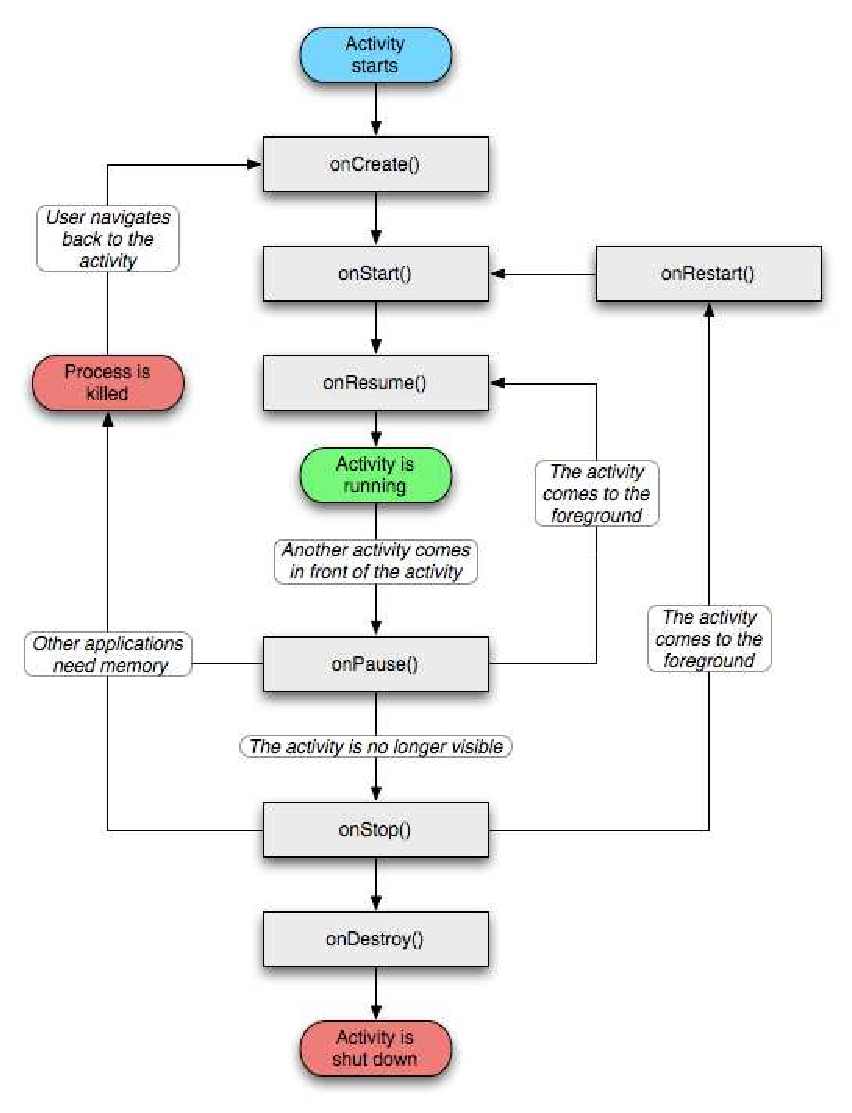
\includegraphics[scale=0.8]{Images/activityLifecycle.pdf}
  }
  \caption{Android Activity Life Cycle\protect\footnotemark}
  \end{figure}
  \end{center}
\footnotetext{http://developer.android.com/reference/android/app/Activity.html}
\newpage
 L'affichage de l'activité \textit{Home} est décrit ci-dessous, nous pouvons
 y retrouver une liste personnalisée contenant :
 \begin{itemize}
   \item L'identifiant unique de la caméra,
   \item Suivi de son descriptif,
   \item Puis en indication son URL.
 \end{itemize}
 Nous pouvons également voir en bas de l'image le menu qui apparaît lors de
 l'appui sur la touche menu du téléphone.\newline
 \begin{center}
 \begin{figure}[H] 
  \label{homeScreenShot}
  \centering
  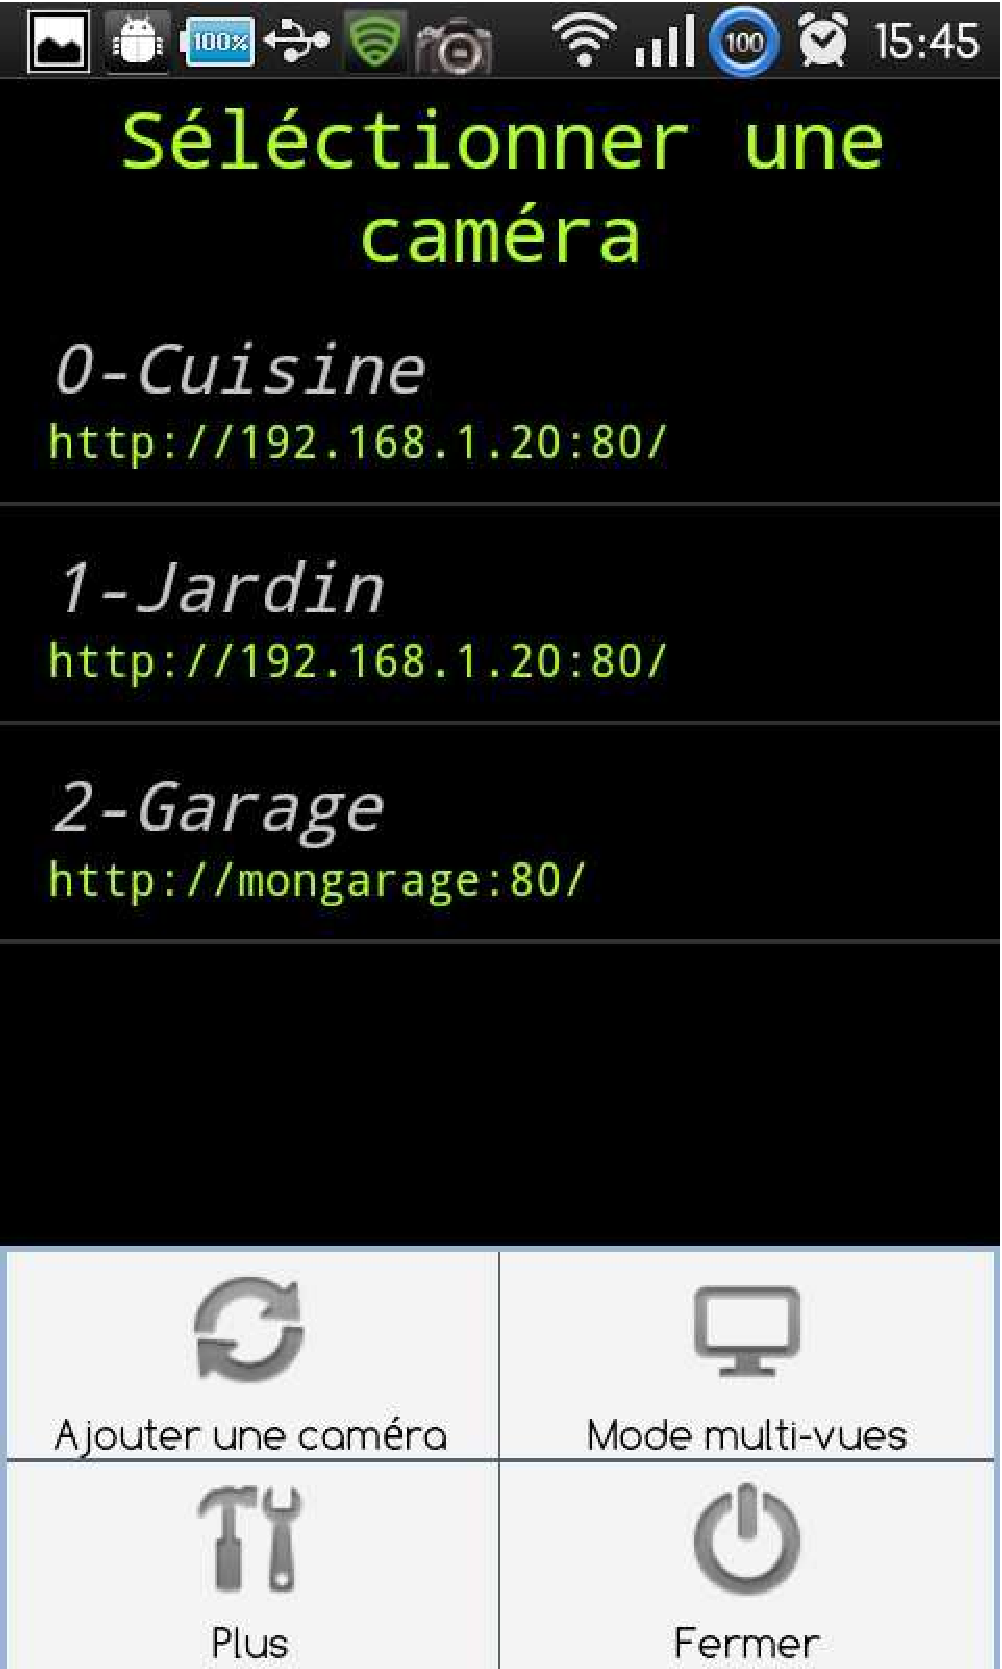
\includegraphics[scale=0.3]{Images/homeScreenShot.pdf}
  \caption{Home SnapShot}
\end{figure}  
\end{center}

\subsection{Modification et Suppression de l'objet}
Lors d'un appui long sur un élément de la liste
(\textit{setOnItemLongClickListener}), une alerte apparaît pour demander à
l'utilisateur s'il souhaite modifier ou supprimer l'élément (la caméra).
\begin{itemize}
  \item S'il choisit de supprimer l'élément, une seconde alerte apparaît pour
  confirmer ou annuler son choix. 
\item S'il choisit de modifier la caméra, l'application lance une nouvelle
activité adaptée à la modification de la caméra. Il peut alors appliquer ou
annuler ses changements sur le même principe que l'ajout d'une caméra.
\end{itemize}
\newpage
\begin{changemargin}{0cm}{0cm}
\begin{lstlisting}[caption={Gestion d'un appui long sur un élément de la
liste.}]
public boolean onItemLongClick(AdapterView<?> arg0, 
			View arg1, final int position, long arg3) { 
	AlertDialog alert; 
	AlertDialog.Builder builder = new AlertDialog.Builder(activity);
	builder.setMessage(getString(R.string.messageChoose))
		.setCancelable(false)
		.setPositiveButton(getString(R.string.boutonModifier),
			new DialogInterface.OnClickListener() {
				@Override
				public void onClick(DialogInterface dialog, int id) {
					Intent intent = new Intent(activity.getApplicationContext(),EditCam.class); 
					Bundle objetbunble = new Bundle();
					objetbunble.putSerializable(getString(R.string.camTag),camList.get(position));
					intent.putExtra(getString(R.string.camPosition), position);
					intent.putExtras(objetbunble);
					dialog.cancel();
					startActivityForResult(intent,EDIT_CODE);
		}}).setNegativeButton(getString(R.string.boutonSupprimer),
			new DialogInterface.OnClickListener() {
				@Override
				public void onClick(DialogInterface dialog, int id) {
					removeCam(position);
					dialog.cancel();
		}});
		alert = builder.create();
		alert.show();
		return true;
}
\end{lstlisting}
\end{changemargin}


\section{Communication avec la caméra}
\subsection{Envoi de requêtes HTTP}
Afin de communiquer avec la caméra, Axis met à disposition des développeurs une
API nommée \textit{VAPIX\footnote{\label{vapix}
http://www.axis.com/techsup/cam\_servers/dev/cam\_http\_api\_index.php}}. Cette
interface est basée sur le protocole HTTP, permettant un accès aux fonctionnalités de la caméra par de simples URLs. Par exemple, pour lister les paramètres réseau de la caméra nous utilisons l'URL suivante :
\begin{lstlisting}
http://myserver/axis-cgi/admin/param.cgi?action=list&group=Network
\end{lstlisting}
En cas de réussite de la requête, nous recevons la réponse suivante :
\begin{lstlisting}
HTTP/1.0 200 OK\r\n
Content-Type: text/plain\n
\n
root.Network.IPAddress=<adresse ip>\n
root.Network.SubnetMask=<masque reseau>\n
\end{lstlisting}

Certaines requêtes comme le contrôle PTZ de la caméra ne provoquent pas de réponse (code HTTP 200) mais indiquent simplement que la requête a bien été reçue (code HTTP 204), cependant nous ne sommes pas informés de la réalisation de l'action demandée.
Nous avons implémenté le mécanisme de requêtes \textit{HTTP} vers la caméra à l'aide de l'objet \textit{HttpURLConnection} dans la méthode \textit{sendCommand} de la classe \textit{CameraControl}. La commande passée en paramètre est concaténée à l'adresse IP de la caméra pour construire l'URL visée.
Nous initialisons alors une connexion HTTP vers l'URL avant d'ajouter un \textit{timeout} au bout duquel la requête est considérée comme un échec, cette valeur étant paramétrable par l'utilisateur dans les préférences de l'application. Le paquet est également forgé avec le champ \textit{Authorization} qui englobe les identifiants encodés en \textit{base64} pour l'authentification.
Pour cela, nous avons réutilisé la classe existante \textit{base64Encoder}\footnote{\label{base64}http://www.rgagnon.com/javadetails/java-0084.html} et ajouté une méthode qui renvoie les identifiants en \textit{base64} sous la forme \textit{login:password}. Par conséquent, l'authentification est réalisée à chaque requête, même si toutes les actions ne nécessitent pas de droits spécifiques.
La méthode retourne enfin l'objet \textit{HttpURLConnection} qui pourra être utilisé pour analyser la réponse et récupérer le contenu avec \textit{getInputStream} dans le cas d'une capture par exemple.

\subsection{Chargement de la configuration}
Avant de récupérer le flux vidéo distant, nous utilisons la méthode \textit{loadConfig} dans le constructeur de la classe \textit{CameraControl} afin de récupérer et établir la liste des fonctionnalités supportées par la caméra. Cette méthode permet aussi de récupérer certains paramètres comme les résolutions et formats d'image disponibles.
Le principe est d'envoyer deux requêtes à la caméra puis de parser le contenu des réponse pour remplir les deux tableaux d'entiers suivants :
\begin{itemize}
	\item \textit{functionProperties} qui conserve les différentes propriétés des fonctions \textit{PAN}, \textit{TILT}, \textit{ZOOM}, \textit{FOCUS} et \textit{IRIS}.
	\item \textit{currentConfig} qui conserve l'état actuel des fonctionnalités
	représenté par les constantes \textit{NOT\_SUPPORTED}, \textit{DISABLED} ou \textit{ENABLED}.
\end{itemize}
La première requête est envoyée à l'adresse suivante :
\begin{lstlisting}
http://myserver/axis-cgi/com/ptz.cgi?info=1
\end{lstlisting}
Le résultat est un long message texte avec pour chaque ligne une chaîne au format \textit{variable=valeur}.
Il suffit alors de parser ligne par ligne en isolant le mot \textit{variable} et en le comparant avec différentes occurences.
Par exemple, le code suivant récupère les capacités de la caméra pour la fonctionnalité "pan" :
\begin{lstlisting}
if (property.contains("pan")) {
	if (property.contentEquals("pan"))
		functionProperties[PAN] += ABSOLUTE;
	else if (property.contentEquals("rpan"))
		functionProperties[PAN] += RELATIVE;
	else if (property .contentEquals("continuouspantiltmove")) {
		functionProperties[PAN] += CONTINUOUS;
		functionProperties[TILT] += CONTINUOUS;
	}
}
\end{lstlisting}
Les constantes identifiant les différentes capacités possibles sont : \textit{ABSOLUTE}, \textit{RELATIVE}, \textit{DIGITAL}, \textit{AUTO}, \textit{CONTINUOUS}.
A la fin du parsage de la première requête, \textit{currentConfig} est mis à jour pour les fonctionnalités concernées par \textit{functionProperties} avec la boucle suivante :
\begin{lstlisting}
for (int i = 0; i < NB_BASIC_FUNC; i++)
	if (functionProperties[i] > 0)
		currentConfig[i] = ENABLED;
\end{lstlisting}

La deuxième requête est quant à elle envoyée à l'adresse suivante :
\begin{lstlisting}
http://myserver/axis-cgi/admin/param.cgi?action=list&group=Properties.Motion.Motion,Properties.Audio.Audio,Properties.Image
\end{lstlisting}
Le parsage de la réponse permet de mettre à jour la configuration relative à la détection de mouvements, à l'audio et à l'image (résolutions, rotations, formats vidéo).

Une fois le chargement de la configuration effectué, il sera possible de savoir si telle fonctionnalité est supportée et/ou activée par l'appel aux méthodes respectives \textit{isSupported} et \textit{isEnabled}.
De même, \textit{enableFunction} et \textit{disableFunction} permettront de faire varier l'état d'une fonction (\textit{ENABLED}/\textit{DISABLED}). Cependant nous n'avons pas utilisé ces deux dernières méthodes car il n'est pas possible de savoir dans quel état actuel se trouve la caméra pour une certaine fonctionnalité.
En effet, plusieurs personnes pouvant agir tour à tour sur les paramètres de la caméra.

\subsection{Liste des commandes utilisées}
Le tableau suivant présente les différentes commandes distantes que nous avons
utilisées dans notre application Android, associant l'adresse pointée (basée toujours sur l'adresse IP de la caméra) à l'action effectuée par la caméra. \begin{table}[H]
\centering
\begin{tabular}{|p{0.5\linewidth}|p{0.5\linewidth}|}
\hline
Partie variable URL & Action
\hline
axis-cgi/com/ptz.cgi?info=1 & Retourne la liste globale des capacités fonctionnelles de la caméra
\hline
axis-cgi/admin/param.cgi?action=list\\\&group=Properties... & Retourne l'état
actuel des paramètres spécifiés (Motion, Audio, Image, \dots)
\hline
axis-cgi/mjpg/video.cgi?resolution=<resolution> & Retourne le flux MJPEG de
résolution <resolution>
\hline
axis-cgi/jpg/image.cgi?resolution=<resolution>
& Retourne une capture d'écran de résolution <resolution>
\hline
axis-cgi/operator/param.cgi?action=add&group=Motion&template=motion & Ajoute une
fenêtre de détection de mouvements
\hline
axis-cgi/operator/param.cgi?action=remove&group=Motion.<groupeID> & Supprime une
fenêtre de détection de mouvements existante d'identifiant <groupeID>
\hline
axis-cgi/motion/motiondata.cgi?group=<groupeID> & Retourne à intervalles
réguliers les niveaux de détection de la fenêtre d'identifiant <groupeID>
\hline
axis-cgi/operator/param.cgi?action=update&Motion.M<groupeID>.<param>=<valeur> &
Met à jour les paramètres de la fenêtre de détection d'identifiant <groupeID>
\hline
axis-cgi/operator/param.cgi?action=update&Motion.M<groupeID>.<param>=<valeur> &
Met à jour les paramètres de la fenêtre de détection d'identifiant <groupeID>
\hline
axis-cgi/com/ptz.cgi?<param>=<valeur>
\begin{itemize}
  \item <param> parmi { rpan, rtilt, rzoom, riris, rfocus, rbrightness }
  \item <valeur> une valeur numérique
\end{itemize} &
Effectue l'action <param> correspondante (pan, tilt, zoom, iris, focus) en
appliquant <valeur> de manière relative (calculé à partir de la position actuelle)
\hline
axis-cgi/com/ptz.cgi?<param>=<valeur>
\begin{itemize}
  \item <param> une valeur parmi { autofocus, autoiris, ircutfilter, backlight }
  \item <valeur> une valeur parmi { on, off, auto}
\end{itemize} &
Active/désactive ou met en mode automatique la fonctionnalité <param>
\hline
\end{tabular}
\caption{Liste des commandes HTTP}
\end{table}

\section{Gestion du flux vidéo}
\subsection{Vue Simple}
Cette partie consiste a décrire l'implémentation de la retransmission de la
vidéo d'une seule caméra sur le téléphone. Cette implémentation se trouve dans
la classe \textit{Video.java} qui définit l'activité \textit{Video}.
\subsubsection{Cycle de vie}
Précédemment, nous avons décrit le cycle de vie de l'activité \textit{Home}.
Ici nous avons également ajouté des fonctionnalitées aux différents états afin de
ne pas consommer de ressources inutilement. En effet, lorsque l'activité n'est
plus au premier plan, il est inutile de continuer à retransmettre le flux
vidéo.\newline
C'est également le cas pour l'utilisation du verrou nous permettant d'empêcher
le téléphone de se mettre en veille lors de la retransmission de la vidéo. Le
code suivant illustre l'arrêt de la vidéo et la libération du verrou
(wl) lorsque l'activité n'est pas active.\newline
Il existe plusieurs types de verrous. Pour les utiliser, il faut récupérer une
instance du gestionnaire d'énergie \textit{PowerManager} à l'aide de la
fonction : 
\begin{lstlisting}
 PowerManager pm = Context.getSystemService(Context.POWER_SERVICE).
\end{lstlisting}
Puis il faut demander explicitement la création d'un nouveau verrou
(\textit{PowerManager.WakeLock}) à l'aide de la fonction :
\begin{lstlisting}
 pm.newWakeLock(PowerManager.SCREEN_DIM_WAKE_LOCK,"Tag");
\end{lstlisting}
Ces différents verrous sont définis par le premier argument. Il existe quatre
types de verrous dont les caractéristiques sont définies ci-dessous :\newline
\begin{center}
\begin{tabular}{|l|c|c|c|}
\hline
Flag Value & CPU & Screen & Keyboard \\
\hline
PARTIAL\_WAKE\_LOCK & On* & Off & Off \\
SCREEN\_DIM\_WAKE\_LOCK & On & Dim & Off \\ 
SCREEN\_BRIGHT\_WAKE\_LOCK & On & Bright & Off \\
FULL\_WAKE\_LOCK & On & Bright & Bright \\
\hline
\end{tabular}
\newline
\textit{WakeLock flags table\footnote{\label{wakeLockTable}
http://developer.android.com/reference/android/os/PowerManager.html}}
\newline
\end{center}
Nous avons choisi d'utiliser un verrou \textit{SCREEN\_DIM\_WAKE\_LOCK} afin de
garder l'écran simplement allumé avec une luminosité au minimum et ne pas
consommer excessivement la batterie du téléphone.
\newpage
 \begin{lstlisting}[caption={Video life-cycle}] 
/**
 * Called when Activity start
 */
public void onCreate(Bundle savedInstanceState) {
	super.onCreate(savedInstanceState);
	setContentView(R.layout.video);
	setRequestedOrientation(0);
	
	PowerManager pm = (PowerManager) getSystemService(Context.POWER_SERVICE);
	wl = pm.newWakeLock(PowerManager.SCREEN_DIM_WAKE_LOCK, "My Tags");
	(...)
}
/**
 * Resume video and acquire wakelock when activity resume.
 */
public void onResume() {
	super.onResume();
	wl.acquire();
	if (pause) {
	    mv.resumePlayback();
	    pause = false;
	}
}
 /**
 * Stop video and release wakelock when activity sleep
 */
public void onPause() {
	pause = true;
	wl.release();
	if (mv != null)
	    mv.stopPlayback();
	super.onPause();
}

/**
 * Stop Video before destroy
 */
public void onDestroy() {
	if (mv != null)
	    mv.stopPlayback();
	super.onDestroy();
}
\end{lstlisting}
\subsubsection{ConnectivityManager}
L'accès à internet pour un téléphone disposant d'un système d'exploitation
comme Android se fait par des couches physiques de nature différente. Le débit
est donc fortement dépendant du support utilisé, c'est pourquoi nous faisons
appel à la classe \textit{ConnectivityManager}. Celle-ci permet de
récupérer la nature du support et ansi de définir la résolution de la vidéo à
demander auprès de la caméra. Nous avons principalement distingué deux types de
réseaux : \textit{WiFi} et les autres réseaux mobiles (\textit{3G},
\textit{3G+}, \textit{EDGE}, \ldots). Nous avons alors défini la correspondance
suivante qui nous permet d'obtenir un taux de rafraîchissement correct en \textit{WiFi}
(moyenne de 25 FPS pour une couverture totale), la
résolution minimale étant utilisée pour les autres réseaux:
\begin{center}
\begin{tabular}{|c|c|}
\hline
Réseau & Résolution \\
\hline
WiFi & 320x240\\
Autres & 168x120\\
\hline
\end{tabular}
\newline\newline
\end{center}
Pour récupérer le type de réseau, nous faisons une nouvelle fois appel à
la fonction :
\begin{lstlisting}
ConnectivityManager mConnectivity = (ConnectivityManager) getSystemService(Context.CONNECTIVITY_SERVICE);
\end{lstlisting}
Puis en récupérant une instance du réseau actif :
\begin{lstlisting}
NetworkInfo info = mConnectivity.getActiveNetworkInfo();
if (info != null && info.isConnected()) {
  int netType = info.getType();
  if (netType == ConnectivityManager.TYPE_WIFI) {
	/*... Code pour un support de type WiFi ...*/
  } else {
	/*... Code pour les autres supports ...*/
  }
\end{lstlisting}

\subsubsection{Format Vidéo}
Android est capable d'encoder et de décoder un grand nombre de format audio et
vidéo (cf Android Supported Media Formats\footnote{\label{mediaFormat}
http://developer.android.com/guide/appendix/media-formats.html}) à travers
deux protocoles (\textit{HTTP ou RTSP}).\newline
La caméra mise a notre disposition propose uniquement deux formats vidéo :
\textit{MJPEG} via le protocole \textit{HTTP} et \textit{MPEG4} via le protocole
\textit{RTSP}.\newline Cependant malgré que le système d'exploitation est
capable d'utiliser le protocole \textit{RTSP}, celui-ci ne nous permet pas de
modifier les requêtes afin d'y ajouter l'authentification nécessaire pour la
lecture de la video. Celle-ci est donc accessible uniquement si la caméra
autorise les utilisateurs anonyme à la visionner.\newline Nous sommes donc
limités au protocole \textit{HTTP} dans lequel nous avons expliqué précédemment
la manière dont nous nous authentifions.\newline\newline
Le format \textit{MJPEG} transporté via le protocole \textit{HTTP} n'étant pas géré par le
\textit{mediaPlayer}\footnote{\label{mediaPlayer}
http://developer.android.com/reference/android/media/MediaPlayer.html}, nous
avons dû trouver un autre moyen d'afficher la video.
\subsubsection{MjpegView}
Grâce à la documentation de la caméra\footnote{\label{docAxis}
http://www.axis.com/techsup/cam\_servers/dev/cam\_http\_api\_2.php} on peut
constater que la vidéo est en réalité composée de la succession d'une multitude
d'images. Pour afficher la vidéo il faut donc simplement faire défiler chacune
des images récupérées dans la réponse de la requête permettant d'obtenir le flux de vidéo \textit{MJPEG}.
\newline
Nous avons trouvé sur internet une composant graphique \textit{OpenSource}
appelé \textit{MjpegView}\footnote{\label{MjpegView}
http://www.anddev.org/multimedia-problems-f28/mjpeg-on-android-anyone-t1871-30.html}
réalisant exactement ce traitement.
Nous avons tout de même dû effectuer quelques modifications pour l'adapter à
notre utilisation (comme l'ajout d'une fonction \textit{resumePlayback} pour
redémarrer la lecture de la vidéo par exemple).\newline
Comme chacun des composants graphique, il peut être ajouter dans une activité ou
défini directement dans une vue au format \textit{xml}.\newline
\begin{center}
\begin{lstlisting}[language=XML, format=XML, caption={video.xml}]
<de.mjpegsample.MjpegView.MjpegView
	android:id="@+id/surfaceView1"
	android:layout_width="fill_parent"
	android:layout_height="fill_parent" />
\end{lstlisting}
\end{center}
\begin{center}
\begin{lstlisting}[caption={mjpegViewer.java}] 
public void onCreate(Bundle icicle) {
	super.onCreate(icicle);
	MjpegView mv = new MjpegView(this);
	setContentView(mv);
	mv.setSource(URL);
	mv.setDisplayMode(MjpegView.SIZE_BEST_FIT);
	mv.showFps(true);
	(...)
}
\end{lstlisting}
\end{center}


\subsubsection{Interface de contrôle de la caméra}
Nous avons choisi de mettre à disposition les commandes permettant le contrôle
de la caméra dans cette activité. Ainsi l'utilisateur peut observer instantanément les
modifications.\newline\newline
\indent Le \textit{LayoutInflater} est une service du système d'exploitation qui
permet de charger une vue a partir d'un fichier \textit{.xml}. Nous allons utiliser ce
service pour ajouter, ou supprimer un ensemble de composant graphique à la vue
retransmettant la vidéo.
\begin{lstlisting}[caption={LayoutInflater utilisation}]
RelativeLayout screen = (RelativeLayout) findViewById(R.id.RelativeLayout01);
LayoutInflater inflater = (LayoutInflater) getSystemService(Context.LAYOUT_INFLATER_SERVICE);
/* Add view from mds_video.xml */
inflater.inflate(R.layout.mds_video, screen, true);
/* Remove all component contained in the mainLayout */
screen.removeView(findViewById(R.id.mainLayout));
\end{lstlisting}
Voici les différentes vue produites :

\begin{center}
\begin{figure}[H] 
  \label{videoView}
    \centering
   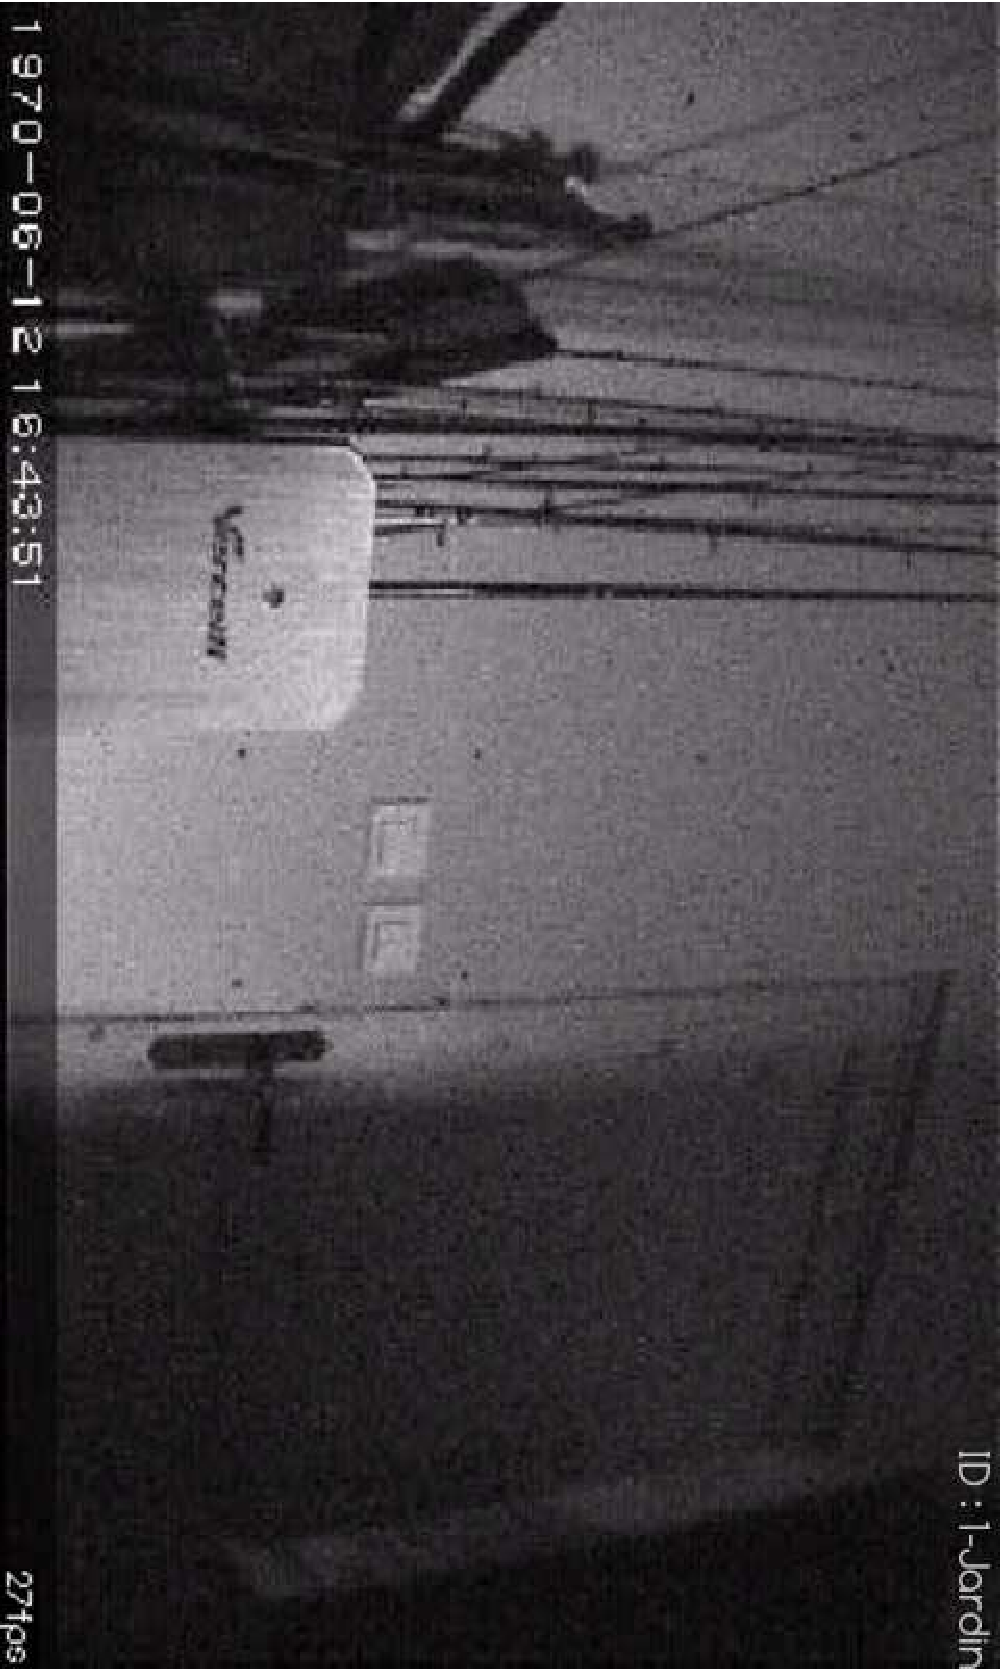
\includegraphics[angle=90,scale=0.3]{Images/videoView.pdf}
  \caption{Minimal view for control video.}
\end{figure}
  
\begin{figure}[H] 
  \label{videoViewAdvC}
    \centering
   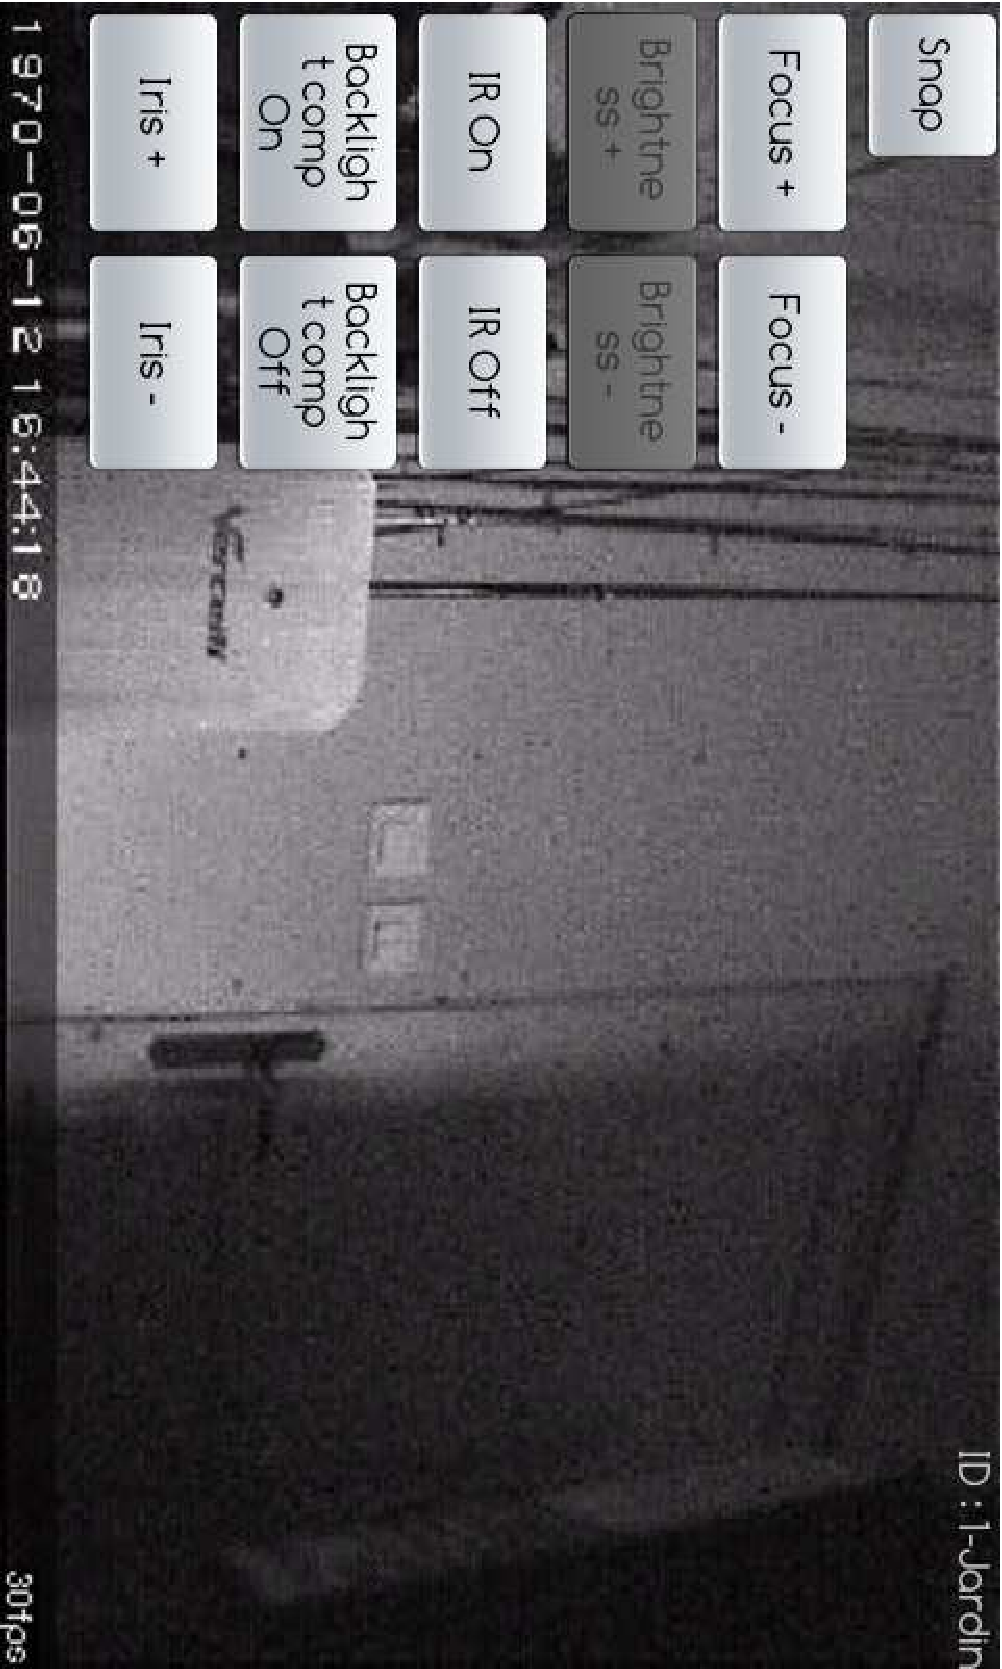
\includegraphics[angle=90,scale=0.3]{Images/videoViewAdvC.pdf}
  \caption{Adding components contained in the file \textit{adv\_video.xml}.}
\end{figure}

\begin{figure}[H] 
  \label{videoViewMD}
  \centering
   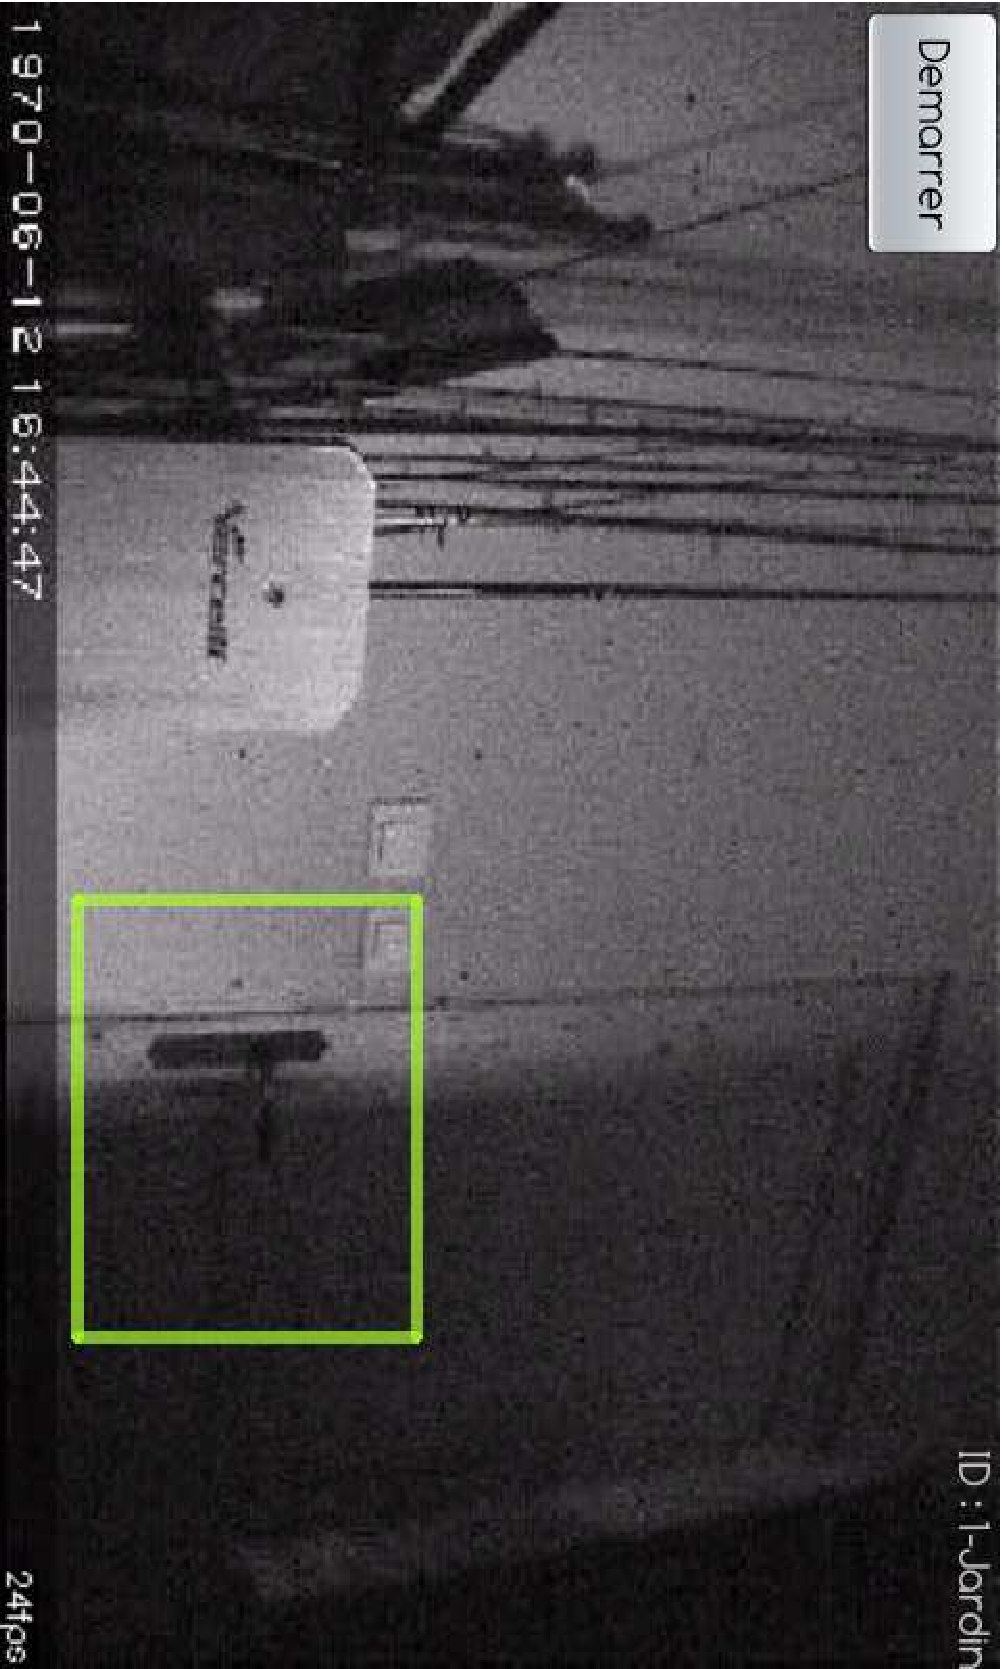
\includegraphics[angle=90,scale=0.3]{Images/videoViewMD.pdf}
  \caption{Adding components contained in the file \textit{mds\_video.xml}}
\end{figure}  
\end{center}

Toutes ces vues peuvent être ajouter ou supprimer en utilisant le menu
personnalisé dans l'activité \textit{Video}.

\subsection{Multi-Vue}
Nous avons souhaité implémenter la possibilité de visionner plusieurs caméras
simultanément sur une même vue. De nouvelles contraintes sont donc apparuent : 
\begin{itemize}
  \item Comment télécharger et afficher plusieurs vidéos \textit{mjpeg}
  provenant de différentes sources ?
  \item Pouvoir choisir le nombre de caméras à afficher.
  \item Comment choisir les caméras ?
  \item Comment contrôler les caméras ?
\end{itemize}

\subsubsection{Playerthread video}
Le thread lancé au démarrage d'une activité est appelé \textit{UI Thread}\footnote{\label{UIThread}
http://davy-leggieri.developpez.com/tutoriels/android/ui-thread/} ou
\textit{User Interface thread}. Le rôle de se thread est d'exécuter le cycle de
vie de l'activité. C'est également lui qui gère les interactions
utilisateurs et l'affichage. Seul l'UI thread peut modifier l'affichage
ou capturer une interaction.\newline 
\indent Pour afficher simultanément plusieurs vidéos, nous devons donc utiliser
plusieurs threads afin d'obtenir un affichage fluide des vidéos.\newline
Chaque thread aura pour tache de télécharger l'image, puis de signaler à l'UI
qu'une nouvelle image est disponible afin d'actualiser
l'affichage.\newline\newline\indent Il existe plusieurs mécanisme pour effectuer
cette notification.\newline
\begin{itemize}
  \item La première méthode est d'enfiler un objet de type
  Runnable, dans la file d'exécution de l'UI à l'aide de la
  fonction : \newline
  \begin{lstlisting}[caption={Example of use runOnUiThread}]
 runOnUiThread(new Runnable() {
 @Override
 public void run() {
	/* Performed by the UI thread */
	imageView[index].invalide();
  }
});  
  \end{lstlisting}
\item Une autre méthode consiste à notifier l'UI à l'aide de
\textit{Message} grâce à la mise en place d'un \textit{handler} qui
exécute une action pour chaque message reçu.\newline
\begin{lstlisting}[caption={Example of message handler}] 
/* Performed by the UI thread */
public static Handler myViewUpdateHandler = new Handler() {
  public void handleMessage(Message msg) {
	if (msg.what == GUIUPDATEIDENTIFIER) {
		/* Uptdate View message */
		imageView[index].invalide();
	}
	if (msg.what == URLERRORIDENTIFIER) {
		/* Other message type */
	}
	super.handleMessage(msg);
}};    
\end{lstlisting}    
\end{itemize}
Le diagramme suivant décrit l'exécution de l'activité \textit{MultiVideo}. A
noter la présence d'un délai entre chaque téléchargement d'une nouvelle image.
Ce délai nous permet de ralentir le nombre d'image par seconde dans le but de réduire considérablement la consommation de la bande passante.
L'utilisateur à la possibilité de régler lui même ce délai dans le menu des
paramètres.
 \begin{figure}[H]
  \label{DiagrammeSequenceMultiView}
  \centering
   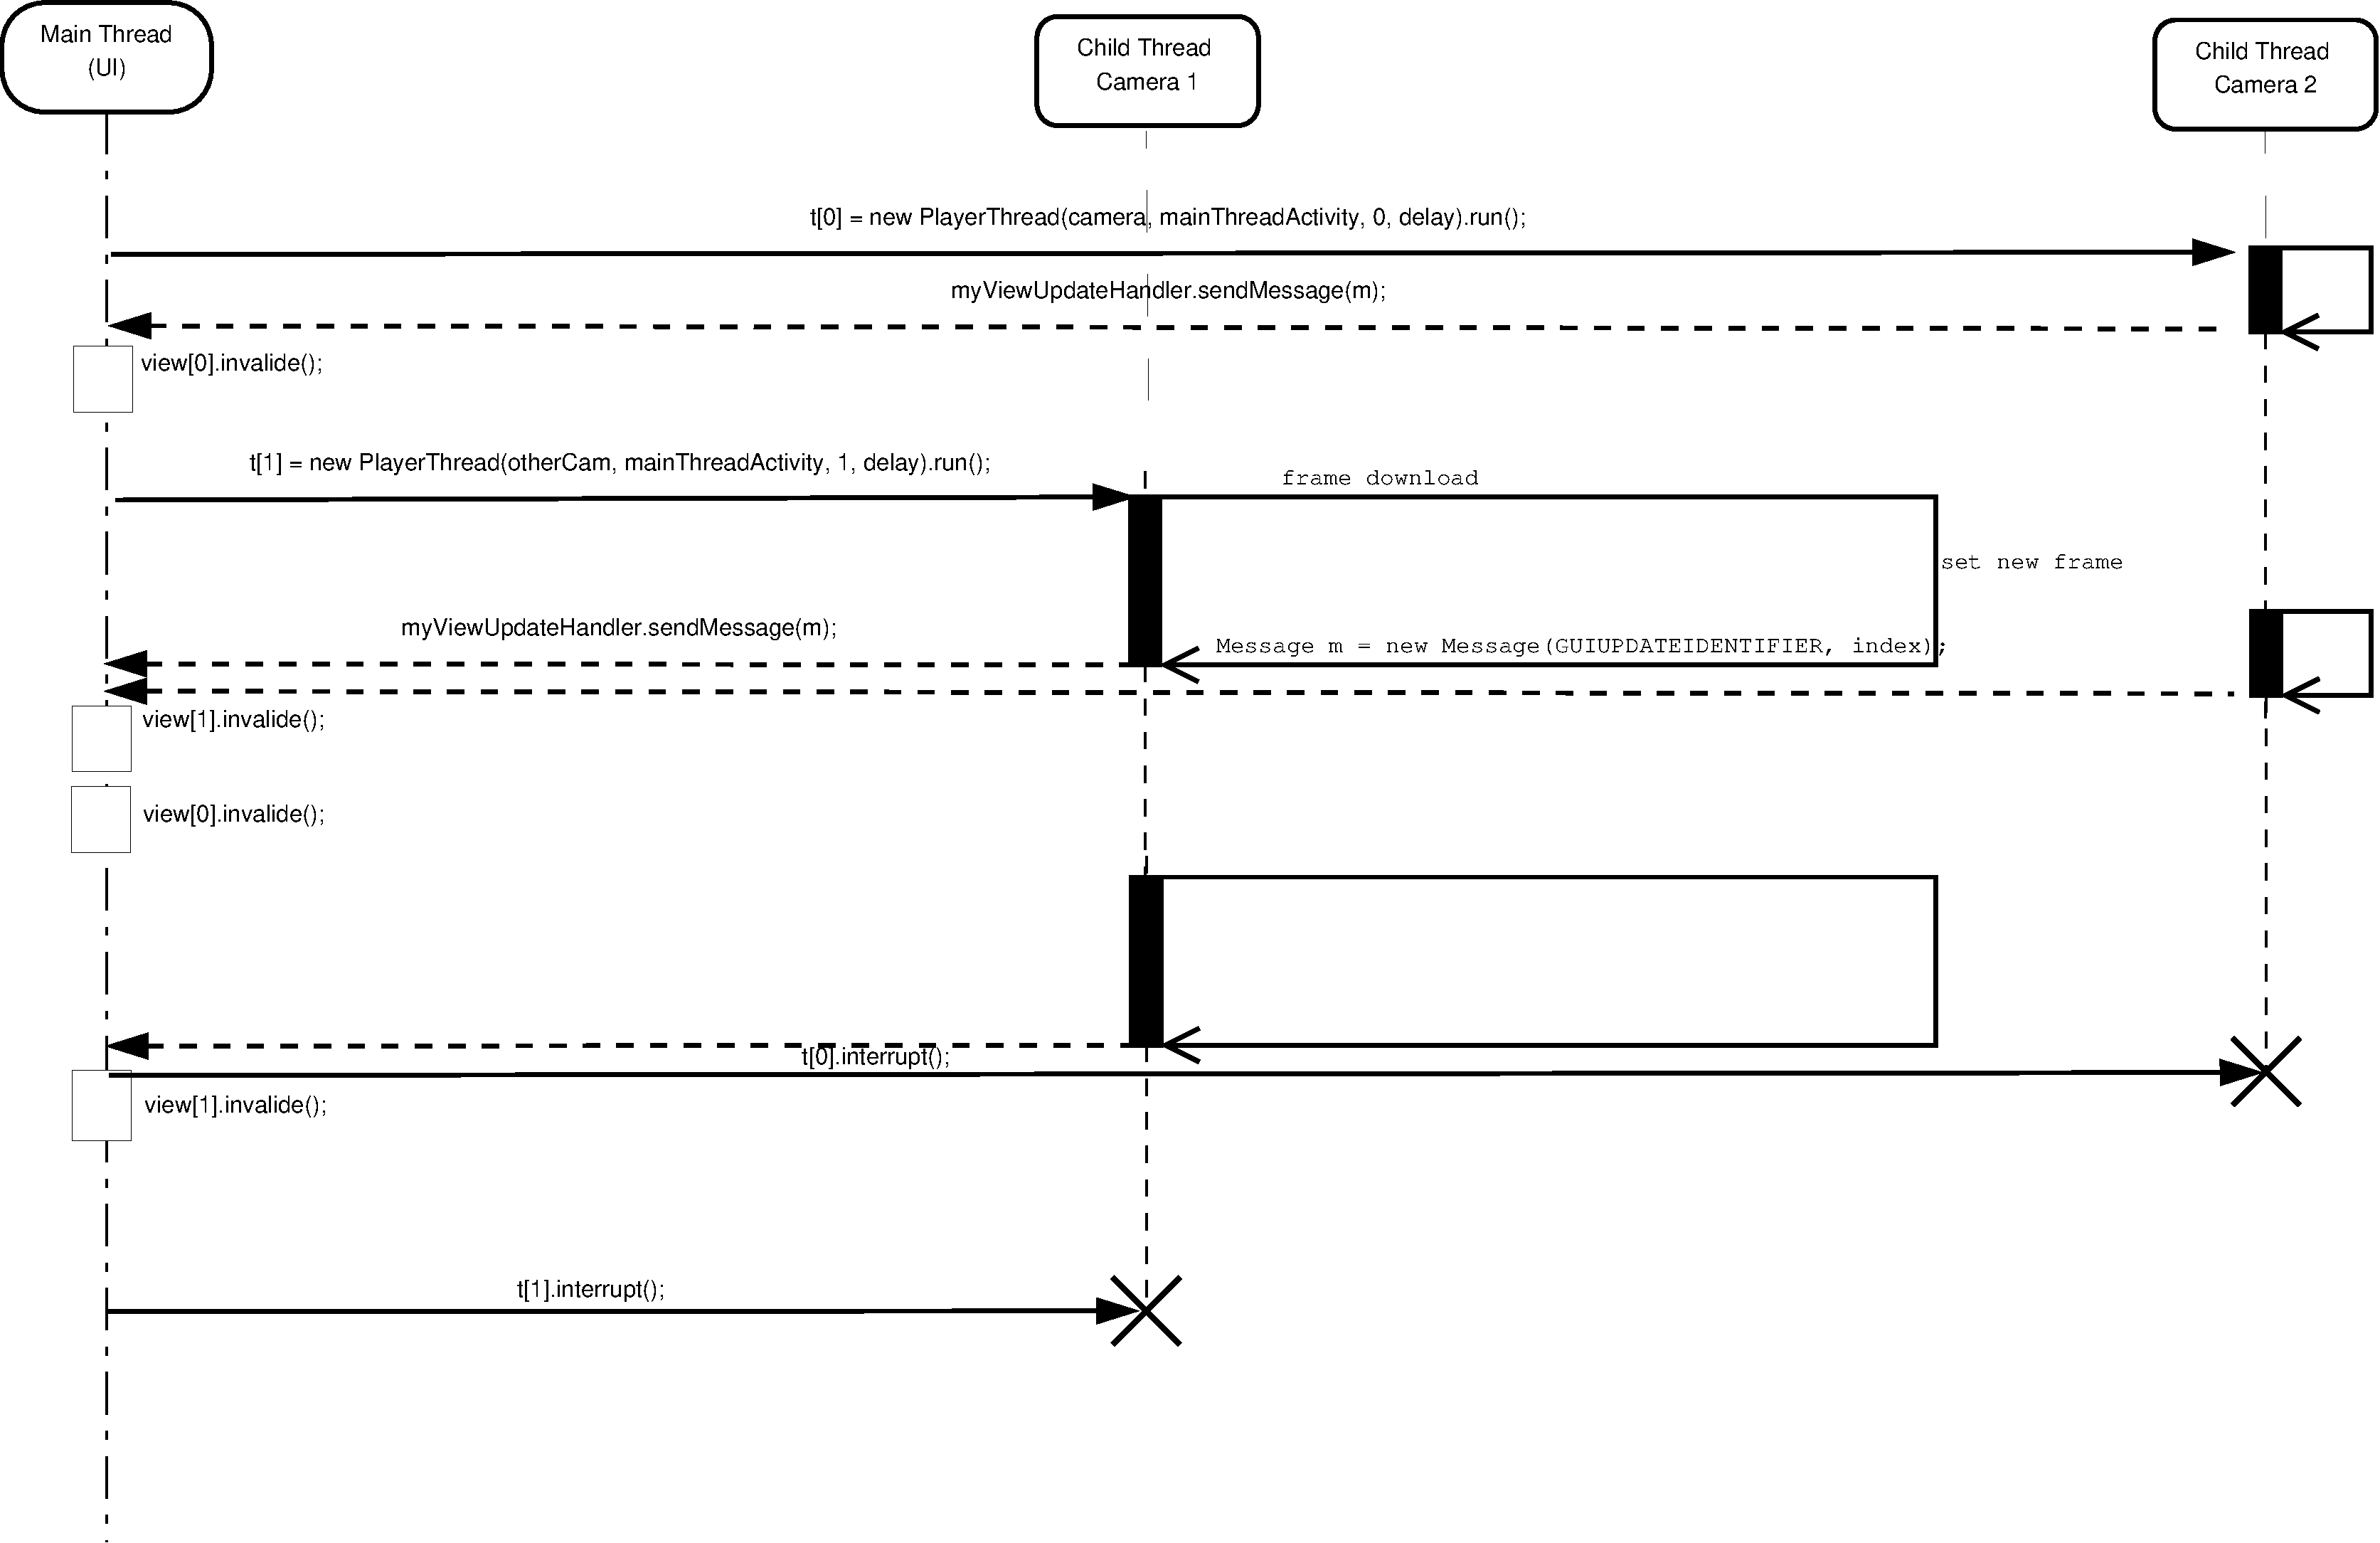
\includegraphics[scale=0.22]{Images/DiagrammeSequenceMultiView.pdf}
  \caption{Multi-View sequence diagram}
\end{figure}  


\subsubsection{Layout personnalisés}
Maintenant que vous sommes capable d'afficher plusieurs vidéos simultanément,
nous nous sommes intéressés à la disposition de celles-ci sur l'écran.
Pour sa faire nous offrons dans un premier temps à l'utilisateur la possibilité
de choisir le nombre de caméra à afficher (entre 2 et 6).\newline
Ceci à l'aide d'un alert dialog qui affichera sous forme d'une liste, le nombre
de caméra à afficher. Puis lors de la capture d'un clic sur l'un des éléments de
la liste, nous lancerons l'activité \textit{MultiVideo} en y ajoutant un
paramètre supplémentaire appelé \textit{nbViewTag} qui défini le nombre de vue
ainsi récupéré.
\begin{changemargin}{0cm}{0cm}
\begin{lstlisting}[caption={Multi-Video launcher}] 
AlertDialog.Builder builder = new AlertDialog.Builder(activity);
builder.setTitle(getString(R.string.cameraAlertTitle));
builder.setSingleChoiceItems(nb_view, -1, new DialogInterface.OnClickListener(){ 
public void onClick(DialogInterface dialog, int item) {
dialog.dismiss();
Intent intent = new Intent(activity,  MultiVideo.class);
Bundle objetbunble = new Bundle();
objetbunble.putSerializable(getString(R.string.camListTag), camList);
intent.putExtras(objetbunble);
intent.putExtra(getString(R.string.nbViewTag),(item + 2));
startActivity(intent);
}
});
AlertDialog alert = builder.create();
alert.show();
\end{lstlisting}    
\end{changemargin}
Enfin dès le lancement de l'activité \textit{MultiVideo}, il ne nous reste plus
qu'à récupérer les paramètres pour définir le layout à utiliser.\\
\newline\indent Nous allons maintenant commenter un problème technique
rencontrer lors de la mise en place des layouts.
Nous avons expliqué précédemment la manière dont nous récupérions le nombre de
caméra à afficher. Afin d'afficher les images récupérées par les différents
threads, nous devons dans un premier temps récépérer chacune des adresses des
différentes \textit{ImageView} défini dans les cinq layout. \newline Pour se
faire, toutes les \textit{ImageView} auront un identifiant défini par leurs
positions sur l'écran :
\begin{itemize}
\item image0 pour le 1er emplacement
\item image1 pour le second
\item image5 pour le 6eme emplacement (le plus grand disponible)
\end{itemize}
En nommant toutes les \textit{ImageView} des différents layout avec un
identifiant équivalent, nous pouvons déduire l'ensemble des adresses en
récupérant celle de l'image0.
En effet lors de la compilation, le compilateur génère un fichier appelé
\textit{R.java}. Dans ce fichier on trouve l'ensemble des adresses pour chaque
classe, layout, et objet de l'application trié par ordre alphabétique. Cette
dernière propriété nous garantie que l'adresse de l'image1 vaut l'adresse de
l'image0 plus un, etc \ldots. Nous sommes donc en mesure de récupérer chacune des 
\textit{ImageView} afin de les mettre a jours, lors de la réception de nouvelle
images mais aussi de définir les \textit{listener} pour chaque images permettant 
de capturer les interactions.
\begin{changemargin}{0cm}{0cm}
\begin{lstlisting}[caption={ImageView address resolver}] 
/*
 * get R.id.image0 address and inc it to find R.id.image1,
 * R.id.image2, ... , R.id.image.n
 */
int dep = R.id.image0;
for (int i = 0; i < nbView; i++) {
img[i] = (ImageView) findViewById(dep + i);
/* Set Image and Listener for each view */
camView[i] = null;
img[i].setImageResource(R.drawable.cadre);
img[i].setOnClickListener(new myOnClickListener(i));
img[i].setOnLongClickListener(new myOnLongClickListener(i));
}
\end{lstlisting}   
\end{changemargin}

 \begin{figure}[H]
  \label{2cam.pdf}
  \centering
   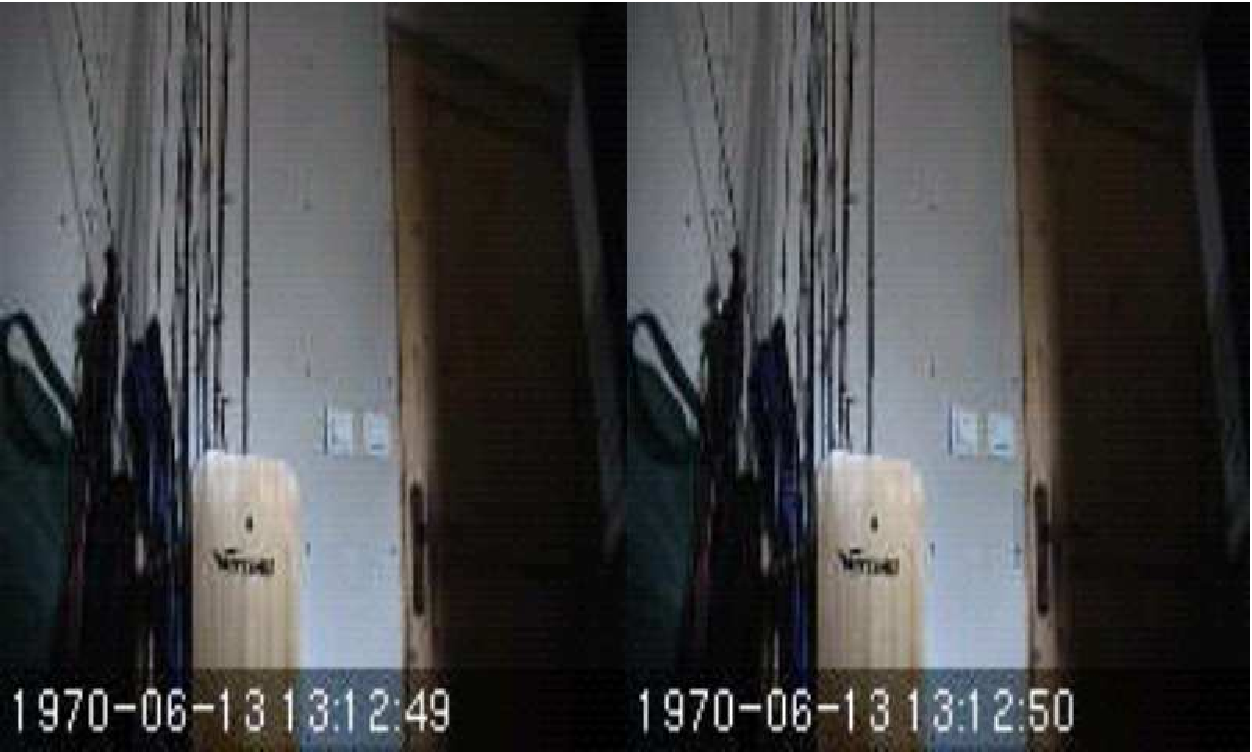
\includegraphics[scale=0.4]{Images/2cam.pdf}
  \caption{Multi-View 2 camera}
\end{figure}  
\begin{figure}[H]
  \label{3cam.pdf}
  \centering
   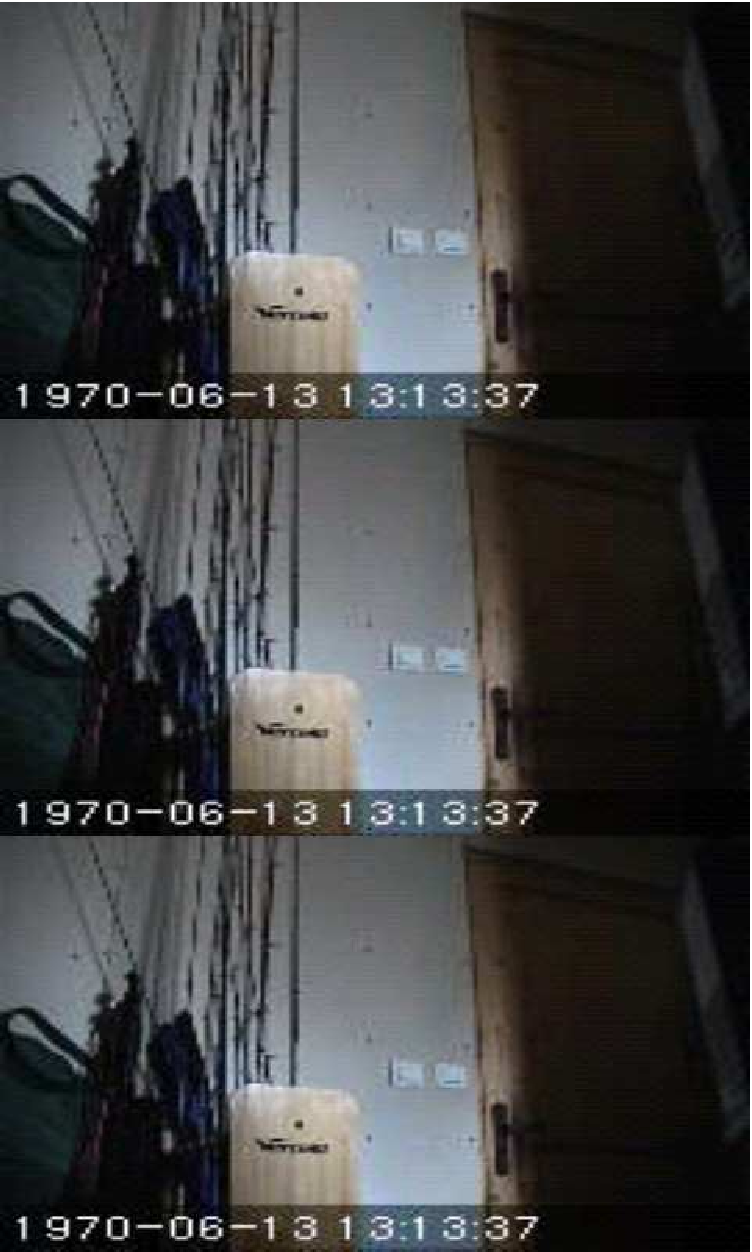
\includegraphics[scale=0.4]{Images/3cam.pdf}
  \caption{Multi-View sequence 3 camera}
\end{figure}  
\begin{figure}[H]
  \label{5cam.pdf}
  \centering
   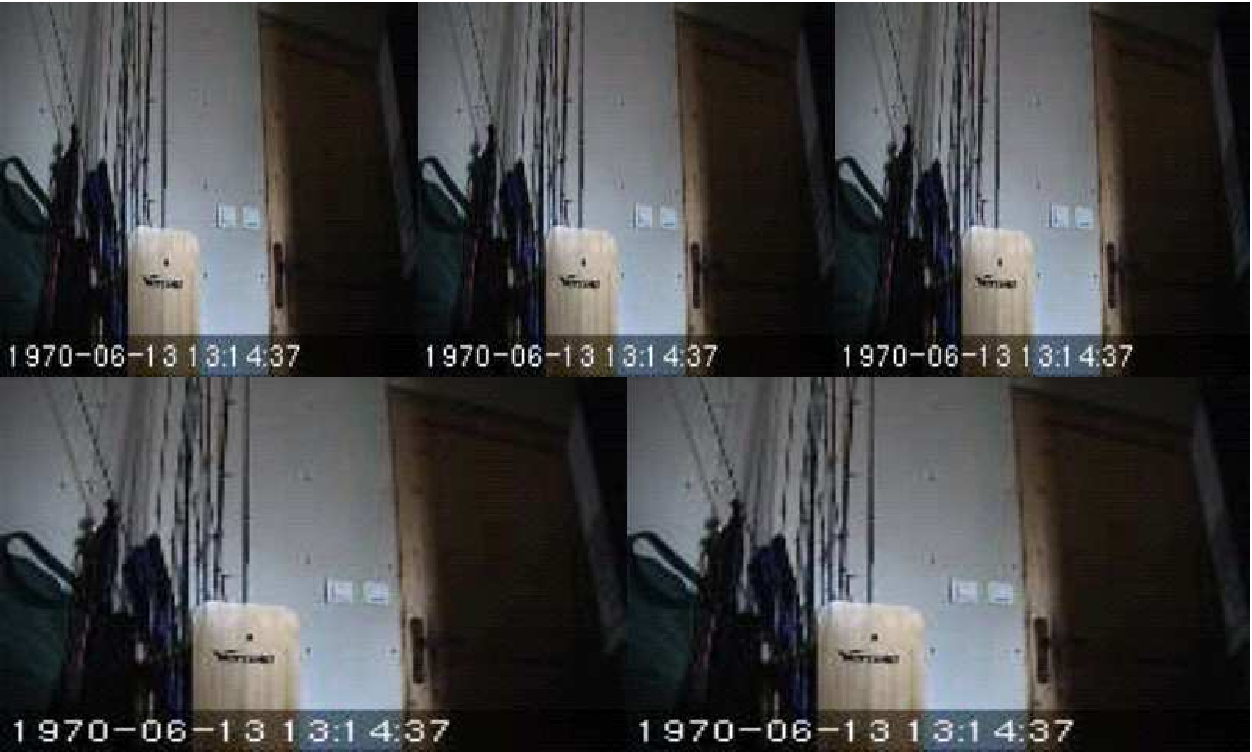
\includegraphics[scale=0.4]{Images/5cam.pdf}
  \caption{Multi-View 5 camera}
\end{figure}  
\subsubsection{Utilisation}
L'utilisateur a également la possibilité de choisir la caméra à afficher sur chacune des \textit{ImageView}. 
\begin{itemize}
\item Le premier clique sur l'une d'elle affiche une liste permettant de
choisir la caméra à afficher.
\item Un nouveau clique stop la vidéo.
\item Un long clique lance l'activité \textit{Video} pour permettre à
l'utilisateur de contrôler la caméra. Une fois les réglages effectuer, il peut
revenir sur la vue précèdente en appuyant sur le bouton retour de son téléphone.
\end{itemize}
Le diagramme d'etat suivant illustre les differents changements d'etat des
videos lorsque l'utilisateur interagi avec l'application. On y retrouve
principalement l'arret de toutes les vidéos lors du passage en simple vue, ainsi
que le redemarrage des vidéos lors du retour de celle-ci.
\begin{figure}[H]
  \label{DiagrammeSequenceMultiView}
  \centering
   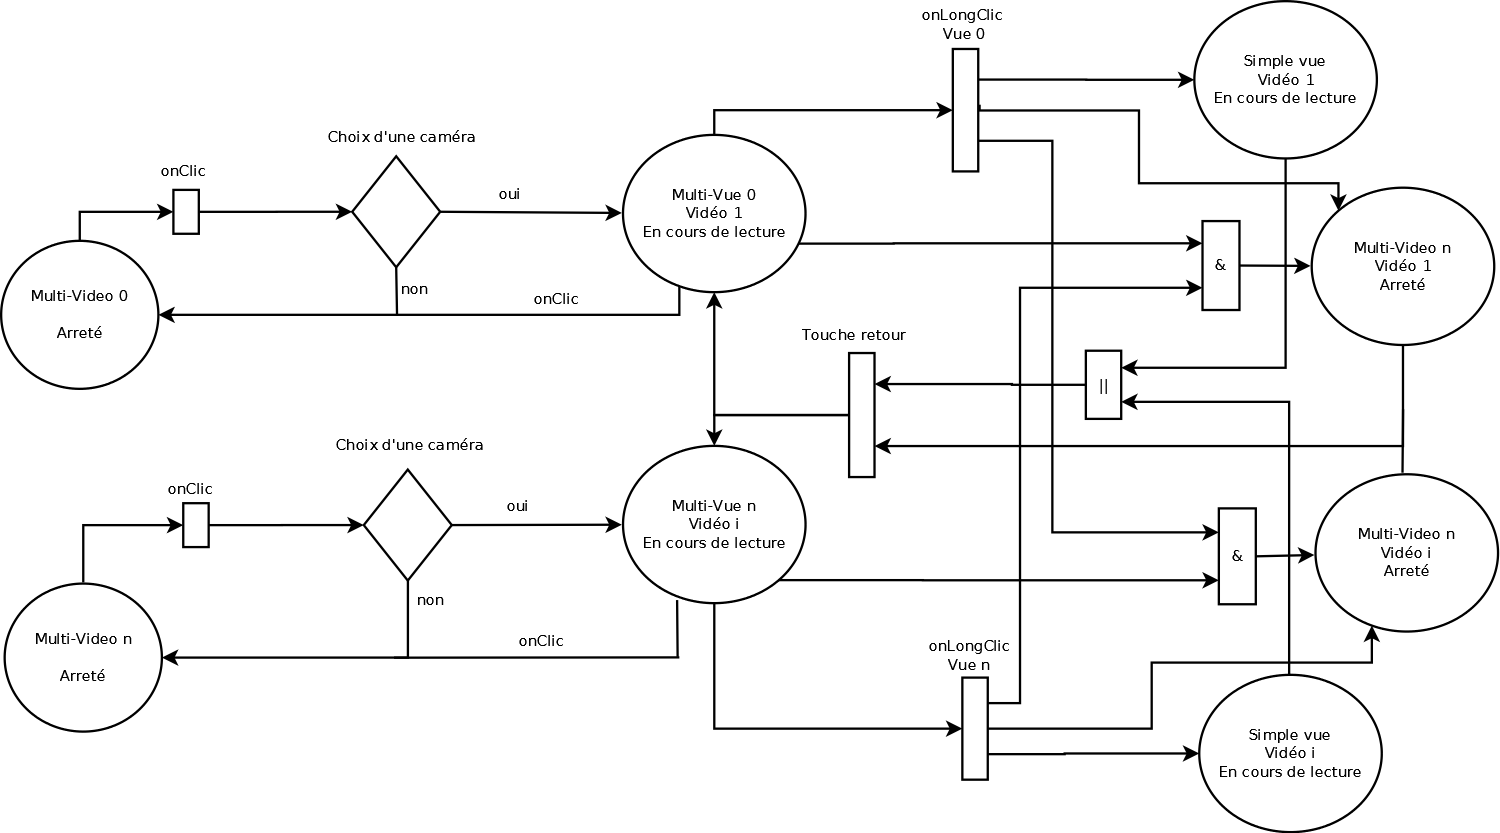
\includegraphics[scale=0.65]{Images/DiagrammeEtatMultiVideo.png}
  \caption{Diagramme d'etat pour une 2-vue.}
\end{figure}  


\section{Contrôle de la caméra}
\subsection{CameraControl}
La communication pour le contrôle du Pan/Tilt/Zoom et des fonctionnalités spécifiques (snapshot, contrôles avancés) de la caméra s'effectuent à travers la classe \textit{CameraControl}.
Les fonctions \textit{changeValFunc} et \textit{switchAutoFunc} permettent d'envoyer les requêtes HTTP à la caméra pour changer la valeur des différents paramètres de celle-ci :
- \textit{PAN}, \textit{TILT}, \textit{FOCUS}, \textit{IRIS}, \textit{BRIGHTNESS} identifient des paramètres prenant une valeur flottante
- \textit{AUTOFOCUS}, \textit{AUTOIRIS}, \textit{AUTO\_IR}, \textit{BACKLIGHT}
identifient des paramètres dont la valeur est comprise dans { \textit{on}, \textit{off}, \textit{auto} } Une réponse HTTP de code \textit{HttpURLConnection.HTTP\_NO\_CONTENT} (code 204)
indique la réussite de la requête, cependant nous ne savons pas si l'action a bien été effectuée.

La fonction \textit{takeSnapshot} réalise la requête de capture d'écran avec comme résolution la valeur passée en paramètre.
Elle retourne les données renvoyées par la caméra sous forme d'un objet \textit{Bitmap}.

Cette classe s'occupe également des activation/désactivation de la détection :
\begin{itemize}
	\item \textit{addMotionD} ajoute une fenêtre de détection.
	\item \textit{removeMotionD} supprime une fenêtre de détection existante.
	\item \textit{updateMotionDParam} met à jour certains paramètres de la fenêtre
	de détection comme les coordonnées ou la sensibilité de détection.
\end{itemize}

Lors du chargement du menu et du layout des contrôles avancés de la caméra, nous vérifions si les fonctionnalités correspondantes sont supportées et/ou activées à l'aide des fonctions
\textit{isSupported} et \textit{isEnabled}. Un appui sur les boutons du menu (celui-ci apparaissant lors de l'appui sur la touche "Menu") déclenchera une alerte texte si la fonctionnalité n'est pas
disponible, alors que pour le layout des contrôles avancés nous définissons la disponibilité de la fonctionnalité directement par l'état du bouton (activé/désactivé).

\subsection{TouchListener}
Le contrôle du PTZ tactile a été implémenté à l'aide de la classe \textit{TouchListener}. Nous avons défini deux gestes possibles avec un ou plusieurs pointeurs (doigt, stylet, ...) pour notre application :
\begin{itemize}
\item un déplacement avec un seul pointeur pour faire bouger la caméra (Pan/Tilt)
\item un écartement/rapprochement de deux pointeurs pour zoomer/dézoomer
\end{itemize}
Cette classe implémente l'interface \textit{OnTouchListener} fournissant une fonction \textit{onTouch} dans laquelle nous gérons chaque mouvement du ou des pointeurs à partir d'un objet \textit{MotionEvent}. Un geste sous Android est défini par une suite de mouvements de type \textit{MotionEvent}.
Il existe une dizaine de types d'actions possibles pour \textit{MotionEvent}, cependant nous utilisons seulement les 4 suivants pour notre application :
\begin{itemize}
\item \textit{ACTION\_DOWN} : le premier pointeur a été ajouté (le geste est
commencé) et l'événement contient les coordonnées du pointeur
\item \textit{ACTION\_POINTER\_DOWN} : un nouveau pointeur a été ajouté
\item \textit{ACTION\_POINTER\_UP} : un pointeur a été enlevé
\item \textit{ACTION\_UP} : le dernier pointeur a été enlevé (le geste est
terminé) et l'événement contient les coordonnées du dernier pointeur
\end{itemize}
A partir de ces types d'actions, nous pouvons définir le déplacement de la
caméra par la suite \textit{ACTION\_DOWN - ACTION\_UP} et la gestion du zoom par
la suite : \\ \textit{ACTION\_DOWN - ACTION\_POINTER\_DOWN - ACTION\_DOWN\_UP -
ACTION\_UP} (nous considérons cependant que le zoom n'est réalisé qu'à partir de l'événement
\textit{ACTION\_POINTER\_DOWN}).

Le champ \textit{mode} contient l'état actuel du geste, soit une des constantes \textit{NONE}, \textit{DRAG} ou \textit{ZOOM}.
Nous récupérons également les dimensions de la vue par \textit{getWidth} et \textit{getHeight} pour la mise à l'échelle des distances de déplacements. 
Pour représenter les coordonnées des pointeurs, nous avons utilisé le type \textit{PointF}.

Nous avons implémenté dans cette classe des méthodes de calcul géométrique entre deux objets \textit{PointF} :
\begin{itemize}
	\item \textit{calculateMoveX} pour la différence en abscisse.
	\item \textit{calculateMoveY} pour la différence en ordonnée.
	\item \textit{calculateDistance} pour la distance géométrique.
\end{itemize}

Nous avons également développé des méthodes pour mettre à l'échelle le déplacement des pointeurs sur l'écran par rapport au déplacement réel réalisé par la caméra :
\begin{itemize}
	\item \textit{scaleMoveX} pour le déplacement en abscisse, en utilisant la
	largeur de l'écran \textit{getHeight}.
	\item \textit{scaleMoveY} pour l'échelle en ordonnée, en utilisant la hauteur
	de l'écran \textit{getWidth}.
	\item \textit{scaleZoom} pour le zoom/dézoom, en utilisant \textit{zoomStep}.
\end{itemize}

Afin de rendre moins ``agressif'' le déplacement sur le téléphone, nous avons
mis en place un paramètre de sensibilité, celui-ci étant modifiable dans les préférences.
Le thread est également endormi quelques millisecondes afin d'éviter la
surcharge d'événements à traiter.
Le tableau ci-dessous montre le traitement
réalisé par la méthode \textit{onTouch} dont le code est présenté après.\newline
\begin{table}[H]
\centering
\begin{tabular}{|p{0.2\linewidth}|p{0.4\linewidth}| p{0.4\linewidth}|}
\hline
Type ACTION & Geste du déplacement & Geste du zoom \\
\hline
DOWN & Mise en mémoire des coordonnées du point de départ &  \\
 & \textit{mode = DRAG} & \\
POINTER\_DOWN & & Calcul et mise en mémoire de la distance de départ \\
 & & \textit{mode = ZOOM} \\
POINTER\_UP & & Calcul et mise en mémoire de la distance d'arrivée \\
UP & Calcul des déplacements horizontaux et verticaux & Calcul du ratio entre les deux distances \\
 & Mise à l'échelle des déplacements & Mise à l'échelle du ratio (avec le champ \textit{zoomStep}) \\
 & \textit{mode = NONE} & \textit{mode = NONE} \\
\hline
\end{tabular}
\caption{Algorithme de traitement onTouch}
\end{table}

\begin{lstlisting}
public boolean onTouch(View v, MotionEvent event) {
	width = v.getWidth();
	height = v.getHeight();
	switch (event.getAction() & MotionEvent.ACTION_MASK) {
	case MotionEvent.ACTION_DOWN:
	    current.set(event.getX(), event.getY());
	    mode = DRAG;
	    Log.i(TAG, "mode=DRAG");
	    break;

	case MotionEvent.ACTION_POINTER_DOWN:
	    currentDist = calculateDistance(
		    new PointF(event.getX(0), event.getY(0)),
		    new PointF(event.getX(1), event.getY(1)));
	    mode = ZOOM;
	    Log.i(TAG, "mode=ZOOM");
	    break;

	case MotionEvent.ACTION_POINTER_UP:
	    startDist = currentDist;
	    currentDist = calculateDistance(
		    new PointF(event.getX(0), event.getY(0)),
		    new PointF(event.getX(1), event.getY(1)));
	    Log.i(TAG, "mode=ZOOM(P_UP)");
	    break;

	case MotionEvent.ACTION_UP:
	    if (mode == DRAG) {
		PointF start = new PointF(current.x, current.y);
		current.set(event.getX(), event.getY());
		float moveX = scaleMoveX(calculateMoveX(start, current));
		float moveY = scaleMoveY(calculateMoveY(start, current));
		Log.i(TAG, "move(X,Y):" + moveX + "," + moveY+ "sensibilite / " + sens);
		camC.changeValFunc(CameraControl.PAN, -1* moveX / sens, -1 * moveY
			/ sens);
	    } else if (mode == ZOOM) {
		Log.i(TAG, "startDist=" + startDist);
		Log.i(TAG, "currentDist=" + currentDist);
		if (Math.abs(startDist - currentDist) > 10) {
		    float ratio = (currentDist / startDist > 1) ? currentDist
			    / startDist : -1 * (startDist / currentDist);
		    Log.i(TAG, "ratio=" + ratio);
		    camC.changeValFunc(CameraControl.ZOOM, scaleZoom(ratio), 0);

		}
	    }
	    mode = NONE;
	    Log.i(TAG, "mode=NONE");
	    try {
		/* Bloc UI thread to not spam request */
		Thread.sleep(200);
	    } catch (InterruptedException e) {
		e.printStackTrace();
	    }
	    break;
	}
\end{lstlisting}
\section{Fonctionnalités avancées et réglages}
Les caméras \textit{Axis} offrent un grand nombre de services pour lesquels
nous avons implémenter la possibilité de les utiliser directement avec le
téléphone.
\subsection{Snapshot}
Parmi ces services, la camera propose à l'utilisateur la possibilité de
prendre une photo instantanée. \newline
Pour ce faire il nous suffit d'envoyer une requête \textit{HTTP} à l'adresse
suivante : 
\begin{lstlisting}
http://<servername>/axis-cgi/jpg/image.cgi
\end{lstlisting}
Dans cette requête, nous avons la possibilité d'ajouter de nombreux paramètres
comme la résolution, le taux de compression, l'affichage de la date, l'heure,
etc. Toutes ces options sont décrites dans la documentation de la caméra
\footnote{\label{MjpegView}http://www.axis.com/techsup/cam\_servers/dev/cam\_http\_api\_2.php\#api\_blocks\_image\_video\_jpeg\_snapshot}.
L'image est contenu dans la réponse :
\begin{lstlisting}
HTTP/1.0 200 OK\r\n
Content-Type: image/jpeg\r\n
Content-Length: <image size>\r\n
\r\n
<JPEG image data>\r\n
\end{lstlisting}
Il ne nous reste qu'a convertir le flux en image
à l'aide de la fonction :
\begin{lstlisting}
Bitmap bmp = BitmapFactory.decodeStream(stream);
\end{lstlisting}
puis l'enregistrer dans un fichier :
\begin{lstlisting}
 bmp.compress(Bitmap.CompressFormat.JPEG, 80, fichier);
\end{lstlisting}
Afin de prévenir l'utilisateur de la réception de la capture, nous avons
implémenté une fonction permettant d'ajouter une notification personnalisée dans
la barre de notification du téléphone.\newline
En plus de notifier l'utilisateur, nous lui offrons la possibilité de visionner directement la photo (via le visionneur d'images par defaut) en cliquant sur la notification.
\begin{changemargin}{0cm}{0cm}
\begin{lstlisting}[caption={ImageView address resolver}] 
 public static void statusBarNotificationImage(Activity activity, Bitmap bmp, String text, String path, int id, String tag) {
	NotificationManager notificationManager;
	notificationManager = (NotificationManager) activity.getSystemService(Context.NOTIFICATION_SERVICE);
	Notification notification = new Notification(R.drawable.camera,	"Camera-Axis", System.currentTimeMillis());
	notification.contentView = new RemoteViews(activity.getPackageName(), R.layout.notification);
	/* Notification action (Open gallery) */ 
	Intent intentNotification = new Intent();
	intentNotification.setAction(android.content.Intent.ACTION_VIEW);
	intentNotification.setDataAndType(Uri.fromFile(new File(path)), "image/png");
	PendingIntent pendingIntent = PendingIntent.getActivity(activity.getApplicationContext(), 0, intentNotification, 0);
	notification.defaults |= Notification.DEFAULT_VIBRATE;
	notification.contentIntent = pendingIntent;
	notification.contentView.setImageViewBitmap(R.id.Nimage, bmp);
	notification.contentView.setTextViewText(R.id.Ntext, text);
	notificationManager.notify(tag, id, notification);
    }
\end{lstlisting}   
\end{changemargin}
Ainsi nous obtenons la notification suivante : 
\begin{figure}[H]
  \label{notification}
  \centering
   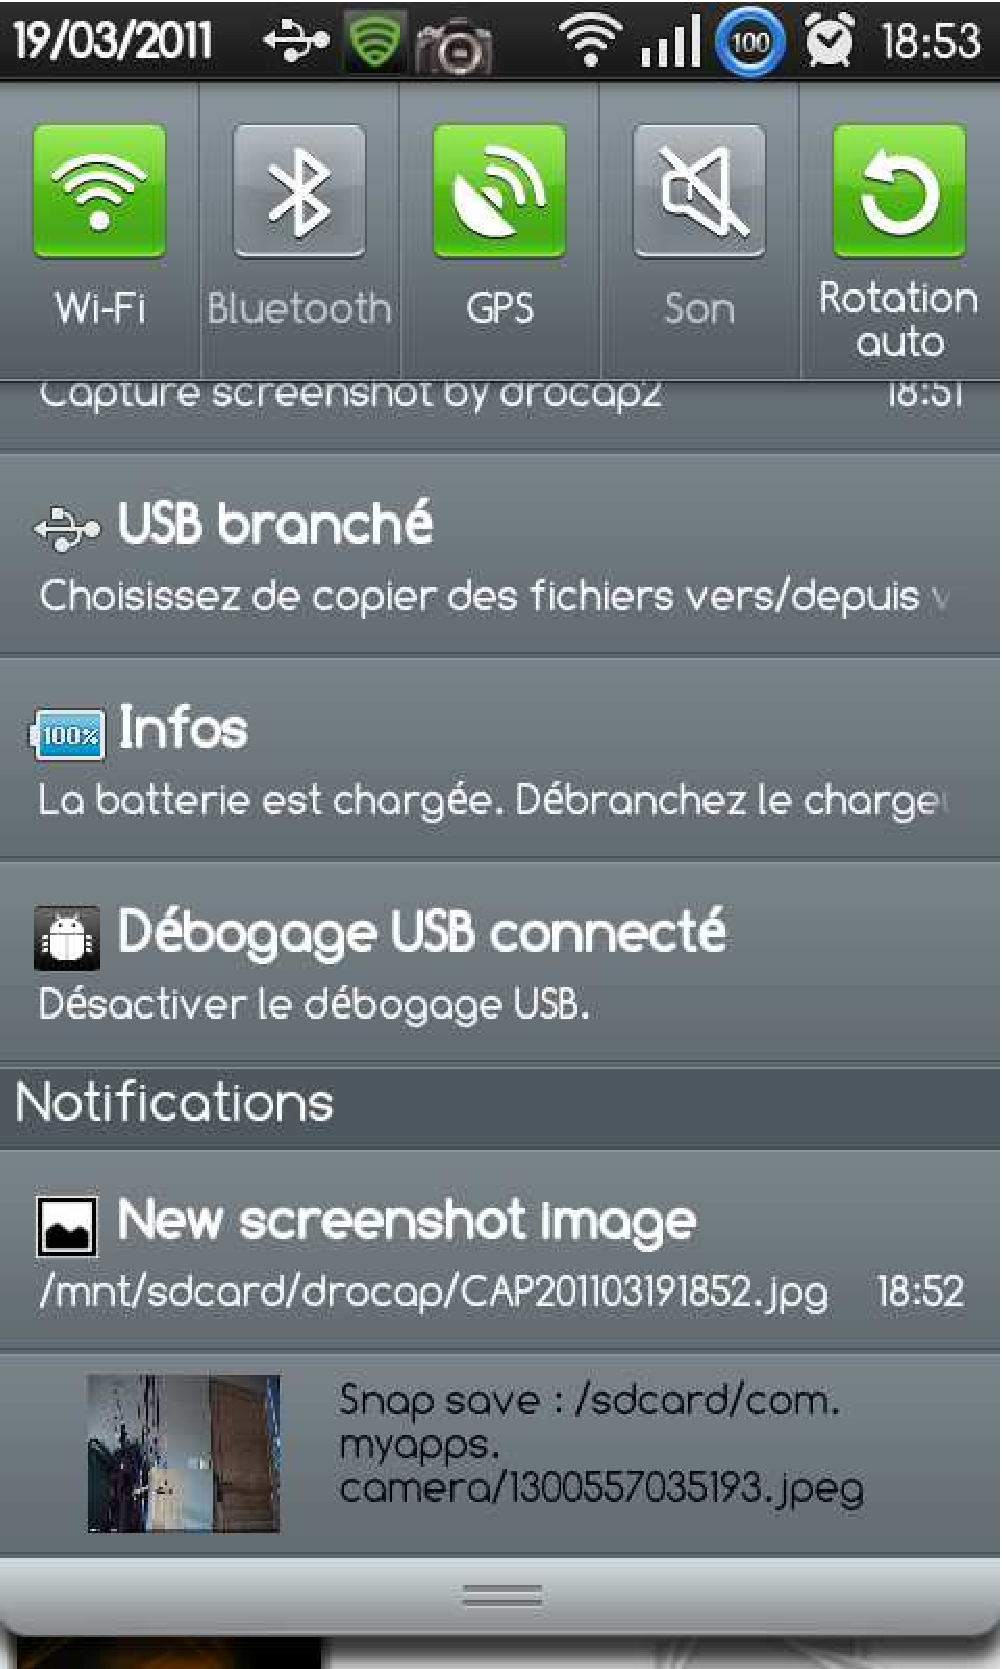
\includegraphics[scale=0.3]{Images/notification.pdf}
  \caption{Notification SnapShot}
\end{figure}  

\subsection{Autres réglages}
Afin d'améliorer la visibilité de la caméra, celle ci propose un grand nombre
de fonction comme le réglage de la luminosité, de la mise au point
(focus), l'ouverture ou la fermeture de l'iris, et beaucoup d'autres fonctions
également disponible sur la
documentation\footnote{\label{MjpegView}http://www.axis.com/techsup/cam\_servers/dev/cam\_http\_api\_2.php\#api\_blocks\_ptz\_control}
de la caméra.\newline
\indent Nous avons choisis d'implémenter certaines d'entre elles dont nous
fournissons l'accès via l'interface de contrôle avancé disponible dans le menu
de l'activité \textit{Video}.

\begin{figure}[H]
  \label{ctrl2}
  \centering
   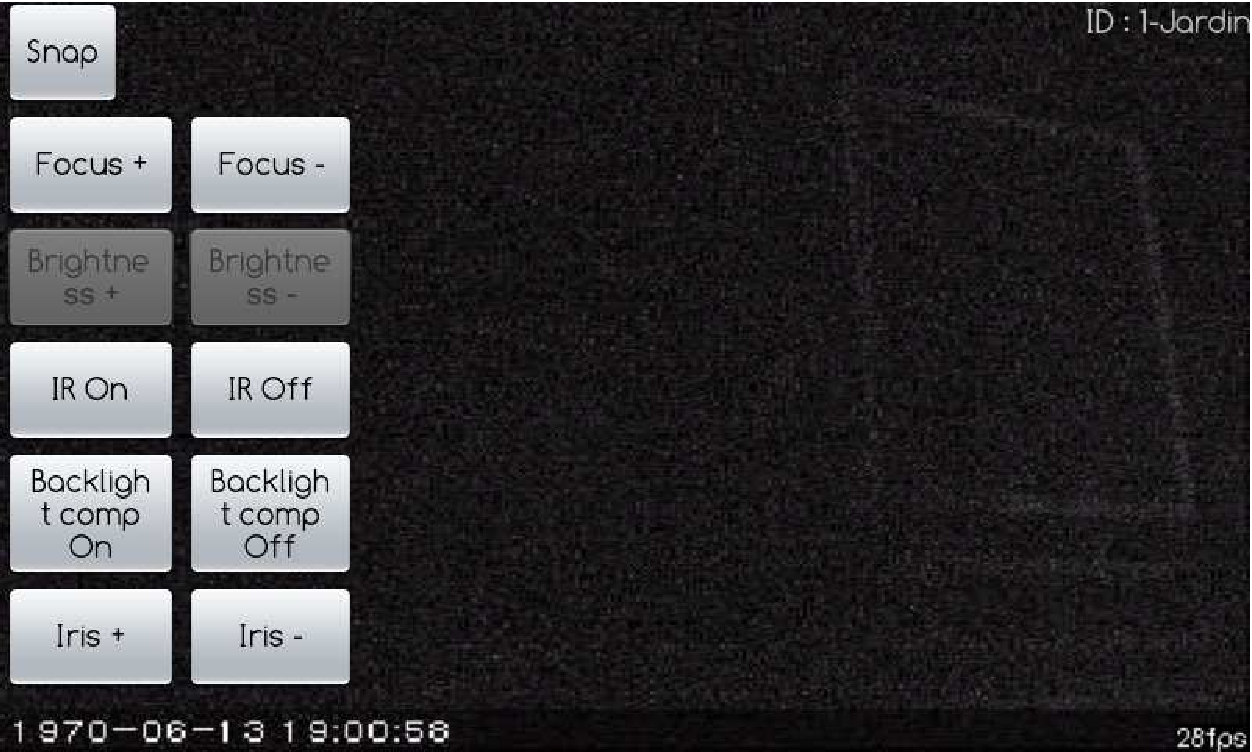
\includegraphics[scale=0.4]{Images/ctrl2.pdf}
  \caption{Advance Controls}
\end{figure}  
\begin{itemize}
  \item \underline{Focus + / Focus - :} Augmenter ou diminuer la mise au
  point.
  \item \underline{Brightness + / Brightness - :} Augmenter ou diminuer la luminosité
  \item \underline{Iris + / Iris - :} Augmenter ou diminuer l'exposition.
  \item \underline{IR On / IR Off :} Activer ou desactiver le filtre
  anti-IR
  \item \underline{Backlight comp On / Backlight comp Off :} Activer ou
  desactiver la correction pour la surexposition à la lumière.
\end{itemize}
Mais nous avons également offert la possibilité à l'utilisateur d'utiliser les
réglages automatique de la caméra toujours à partir du menu de l'activité
\textit{Video}.
\begin{figure}[H]
  \label{ctrl2}
  \centering
   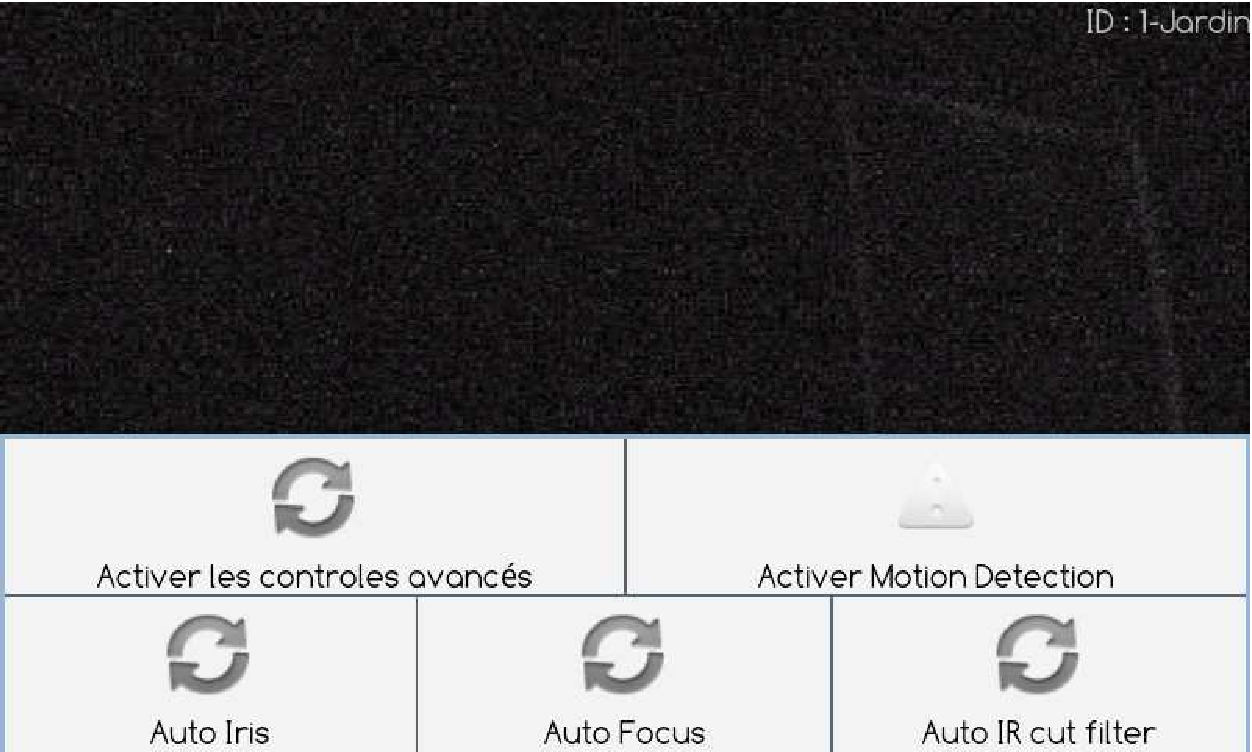
\includegraphics[scale=0.4]{Images/ctrl1.pdf}
  \caption{Advance Controls}
\end{figure}  

\section{Détection de mouvements}
\subsection{Présentation}
La détection de mouvement est une mécanisme utilisé pour détecter les
changements de position, et les mouvements d'objets ou d'individus dans une
zone couverte par un dispositif de video-surveillance.\newline
Selon une traduction de la définition de wikipedia\footnote{\label{MotionDetection}
http://en.wikipedia.org/wiki/Motion\_detection} : \newline
\begin{quotation}
`` Ceci peut être réalisé soit par des dispositifs mécaniques qui interagissent
physiquement avec la zone ou par des dispositifs électroniques qui permettent de
quantifier et mesurer les changements dans l'environnement donné.
Le mouvement peut être détecté par: son (capteurs acoustiques), l'opacité
(capteurs optiques et infrarouges et des processeurs d'images vidéo), le
géomagnétisme (capteurs magnétiques, magnétomètres), la réflexion de l'énergie
transmise (radar laser infrarouges, capteurs ultrasoniques, capteurs et radars
micro-ondes), induction électromagnétique (détecteurs à boucle inductive), et
les vibrations (triboélectrique, sismiques, et des capteurs d'inertie). ``
\end{quotation}
\indent La caméra mise à notre disposition contient un service capable de
détecter les mouvements couvert par l'objectif ou limité à une zone
particulière.\newline Nous avons souhaiter offrir à l'utilisateur la possibilité
de détecter les mouvements et d'en être averti en temps réel sur son téléphone.
C'est pourquoi nous avons implémenté un service à l'écoute de chacune des
caméras afin de détecter les mouvements sans que l'application soit active.
\subsection{Utilisation de service Android}
Sous Android, les services sont des composants qui permettent l'exécution de
fonctionnalités en arrière plan pendant une durée indéterminée même lorsque les
activités de l'application ne sont pas lancée.
Pour créer un service il faut dans un premier temps le déclarer dans le fichier
\textit{AndroidManifest.xml} :\newline
\begin{lstlisting}[format=XML]
<application android:icon="@drawable/camera" 
	android:label="@string/app_name">
	<activity <!-- activities list --> />
	<service android:name="MotionDetectionService" />
</application>
\end{lstlisting}
Puis en implémentant le service dans le fichier
\textit{MotionDetectionService.java}.
 Tout comme les activités, les services ont
un cycle de vie :
\newline
\begin{center}
\begin{figure}[H]
   \label{serviceLifecycle}
  \centering
  \fbox{
  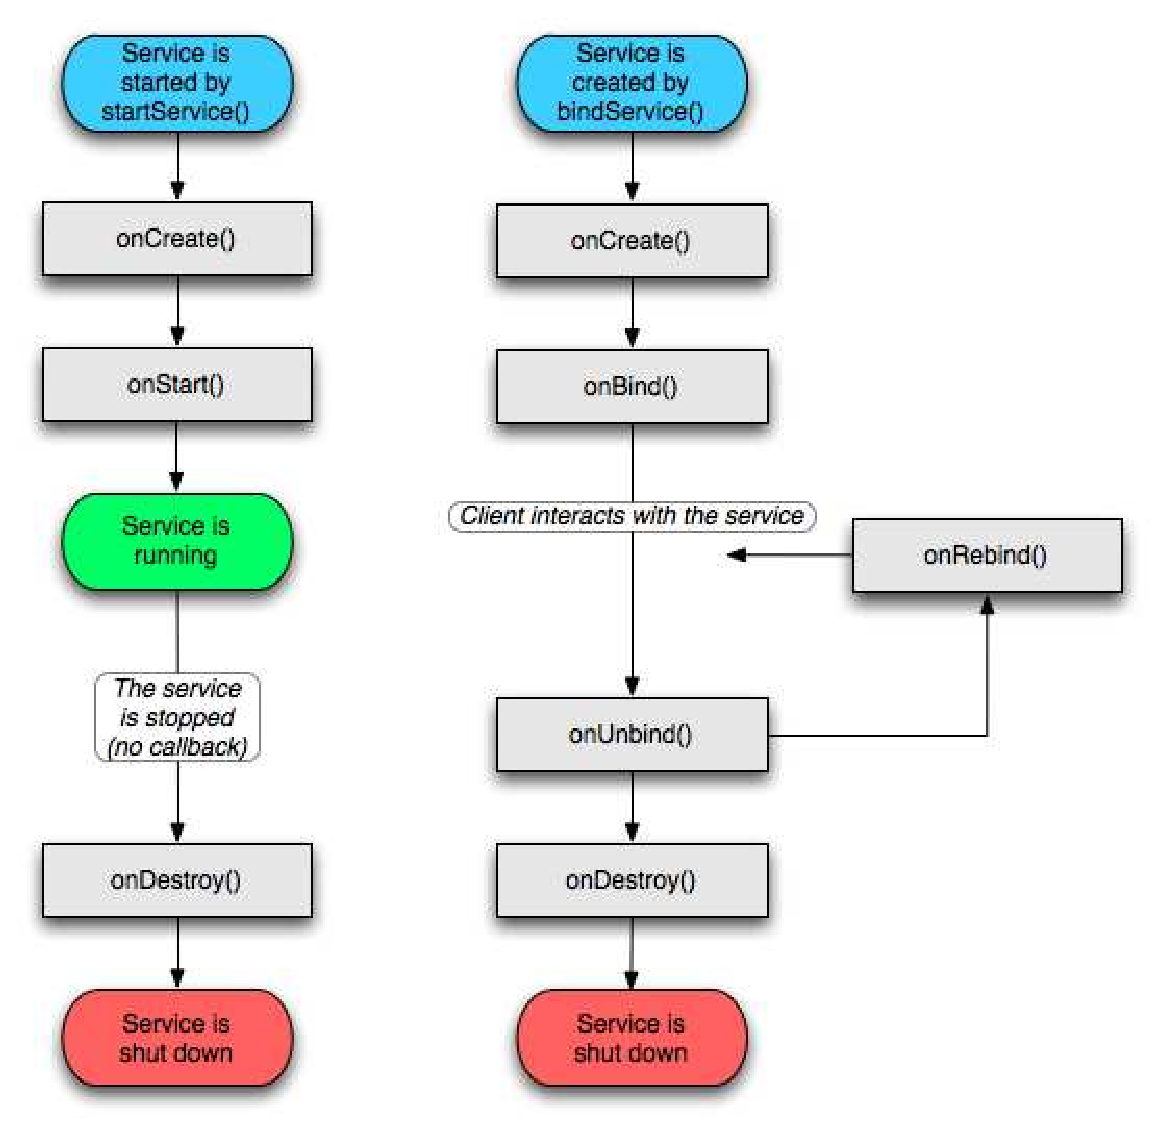
\includegraphics[scale=0.7]{Images/serviceLifecycle.pdf}
  }
   \caption{Service Life Cycle \protect\footnotemark}
  \end{figure}
  \end{center}
\footnotetext{http://www.linuxtopia.org/online\_books/android/devguide/guide/topics/fundamentals.html}

Ce schéma illustre la possibilité de contacter un service de deux manières
différentes. La première (cycle de gauche) se limite à envoyer des instructions 
au service pour y déclencher un traitement défini dans la fonction :
\begin{lstlisting}
@Override
public int onStartCommand(Intent intent, int flags, int startId){
/* work to do */
}
\end{lstlisting}
La seconde (cycle de droite) permet à une activité de se lier à
un service afin de pouvoir utiliser toutes les ses méthodes public.\newline
N'ayant pas besoin de communiquer autrement avec les services que pour leurs
demander d'effectuer un traitement, nous avons choisi d'implémenter le 1er cycle.

\subsection{Activation du service}
Les caméras Axis peuvent gérer jusqu'à dix fenêtres de detection de mouvement par
caméra simultanément. Pour ajouter une fenêtre (avec les valeurs par défaut) il
suffit d'envoyer une requête \textit{HTTP GET} a l'adresse : 
\begin{lstlisting}
http://myserver/axis-cgi/operator/param.cgi?action=add&group=Motion&template=motion
\end{lstlisting}
Pour ajouter une fenêtre défini par sa position sur l'écran, il faut spécifier
explicitement la position de la fenêtre :
\begin{lstlisting}
http://myserver/axis-cgi/operator/param.cgi?action=add&group=Motion&template=motion
&Motion.M.Top=500
&Motion.M.Bottom=7000
&Motion.M.Left=5000
&Motion.M.Right=8500
\end{lstlisting}
Chacune de ces requêtes nous fournira le numéro du groupe (de 0 a 9) associer a
la requête, nous permettant plus tard de recuperer le niveau de la detection.
La réponse est de la forme : 
\begin{lstlisting}
HTTP/1.0 200 OK\r\n
Content-Type: text/plain\r\n
\r\n
M<group number> OK\r\n
\end{lstlisting}
Nous avons de ce fait differencié les détections de mouvement a l'aide d'un entier unique defini tel que : 
\begin{lstlisting}
public int getMotionDetectionID(int startID) {
return groupeID + (uniqueID * 10) + startID;
}
\end{lstlisting}
Chaque caméra dispose d'un numéro unique (sa position dans la liste).
Si elles sont toutes capable de créer dix fenetres de detection, 
en multipliant leur numéro par dix et en additionnant le numero de groupe on peut garantir l'unicité de l'identifiant. Nous ajoutons également un entier \textit{startID} afin de ne pas commencer à compter à partir de zero mais à partir de la valeur contenu dans \textit{startID}.\newline

\indent Pour sélectionner la fenêtre à détecter, nous avons implémenté un nouveau
composant graphique appelé \textit{drawRectOnTouchView} dont la fonction est de
dessiner un rectangle et de récupérer la position de la fenêtre à partir d'un
clique de l'utilisateur.
\subsubsection{drawRectOnTouchView}
Comme pour le lecteur \textit{mjpeg}, l'implémentation d'un nouveau composant
graphique se fait en étendant la classe \textit{View}. Dans une premier temps il
faut définir les constructeurs (Création de la surface sur laquelle dessiner,
définition des couleurs, \ldots). Puis il est nécessaire de surcharger la
méthode :
\begin{lstlisting}
@Override
protected void onDraw(Canvas canvas)
\end{lstlisting}
afin de dessiner le composant. Dans notre utilisation, nous souhaitons dessiner
dynamiquement un rectangle en fonction des interactions fournis par l'utilisateur.
Android nous propose de surcharger une fonction qui est appeler lors de chaque
interactions avec le composant appelé : 
\begin{lstlisting}
@Override
public boolean onTouchEvent(MotionEvent event)
\end{lstlisting}
Grâce a cette fonction, nous allons dessiner un rectangle qui suivra le doigt de
l'utilisateur jusqu'à ce qu'il relâche la pression sur l'écran.
Précédemment nous avons présenté les actions définies par les
\textit{MotionEvent}. Nous allons à nouveau utiliser ces interactions
pour définir le comportement de notre composants :
\begin{lstlisting}[caption={Draw Rectangle Component}] 
@Override
public boolean onTouchEvent(MotionEvent event) {
	float x = event.getX();
	float y = event.getY();
	switch (event.getAction()) {
	case MotionEvent.ACTION_DOWN:
	    start.set(x, y);
	    isDraw = false;
	    break;
	case MotionEvent.ACTION_MOVE:
	    end.set(x, y);
	    isDraw = false;
	    invalidate();
	    break;
	case MotionEvent.ACTION_UP:
	    end.set(x, y);
	    isDraw = true;
	    invalidate();
	    break;
	}
	return true;
    }
    
@Override
    protected void onDraw(Canvas canvas) {
	canvas.drawColor(Color.TRANSPARENT);
	canvas.drawLine(start.x, end.y, end.x, end.y, mPaint);
	canvas.drawLine(end.x, start.y, end.x, end.y, mPaint);
	canvas.drawLine(start.x, start.y, start.x, end.y, mPaint);
	canvas.drawLine(start.x, start.y, end.x, start.y, mPaint);
    }
\end{lstlisting}
Lors de l'appuie sur l'ecran, nous sauvegardons les coordonnées du point, puis
dès le déplacement du doigt de l'utilisateur, on commence à tracer le rectangle.
Enfin lorsque l'utilisateur relève son doigt, on sauvegarde la position du
point, puis on signal que le dessin est dessiné à l'aide du flag
\textit{isDraw}. La fonction \textit{onDraw} nous permet de dessiner les arêtes
du rectangle à partir des coordonnées sauvegardées.\newline
\indent Enfin en affectant la couleur ``transparente'' au fond du composant, on
peut le superposer au dessus d'une vue \textit{mjpeg} pour dessiner un rectangle
sur notre video.\newline
\newline\indent Une fois la détection activée auprès de la caméra, nous pouvons
démarrer notre service en lui indiquant le groupe fournit par la caméra.

\subsection{Détection et Signalisation}
Dans cette partie nous allons étudier le comportement du service.
La detection de mouvement auprès des caméra \textit{Axis} se fait au travers de
la requête GET à l'adresse : 
\begin{lstlisting}
http://myserver/axis-cgi/motion/motiondata.cgi?group=<group number>
\end{lstlisting}
Dans le résultat de cette requête, nous nous intéressons à la valeur du niveau
de detection. Si celui-ci dépasse le seuil défini dans les paramètres
utilisateur, le service déclenche une notification sous forme de vibration du
téléphone ainsi que la prise d'une photo instantannée. La photo sera
alors sauvegardé dans le dossier \textit{"/sdcard/com.myapps.camera/"} sous la
forme : "MD-time-<heure en ns>.jpeg".
\newline Afin de ne pas ``spammer''
l'utilisateur de notification, nous avons décider d'établir un délai minimum entre deux notifications réglable dans les paramètres.
\begin{lstlisting}
HTTP/1.0 200 OK\r\n
Content-Type: multipart/x-mixed-replace;boundary=axismdb\r\n\r\n
--axismdb\r\n
Content-Type:text/plain\r\n\r\n
group=0;level=28;threshold=45;\r\n
group=1;level=43;threshold=25;\r\n
--axismdb\r\n
Content-Type:text/plain\r\n\r\n
group=0;level=54;threshold=45;\r\n
group=1;level=38;threshold=25;\r\n
--axismdb\r\n
Content-Type:text/plain\r\n\r\n
group=0;level=49;threshold=45;\r\n
group=1;level=19;threshold=25;\r\n
--axismdb\r\n
 .
 .
 . 
\end{lstlisting}
\textit{5.4.5 Get the Motion Detection
level\footnote{\label{MotionDetectionDoc}
http://www.axis.com/techsup/cam\_servers/dev/cam\_http\_api\_2.php\#api\_blocks\_motion\_get\_md\_level}.}


\subsection{Implémentation et lancement de la tache}
Le traitement à effectuer pour chacune des détections lancées sera de
``parser'' le contenu de la réponse citée ci-dessus, puis avertir l'utilisateur en cas de mouvement.
Grâce a la fonction \textit{onStartCommand} défini ci-dessus nous somme en
mesure de lancer des threads dont le rôle sera justement d'effectuer ce
traitement (un thread par caméra).\newline Lorsqu'un mouvement sera détecté
par l'un des threads, nous utiliserons le même principe de handler que le
\textit{PlayerThread} pour prévenir le service activant ainsi une notification.
\begin{figure}[H]
  \label{service}
  \centering
   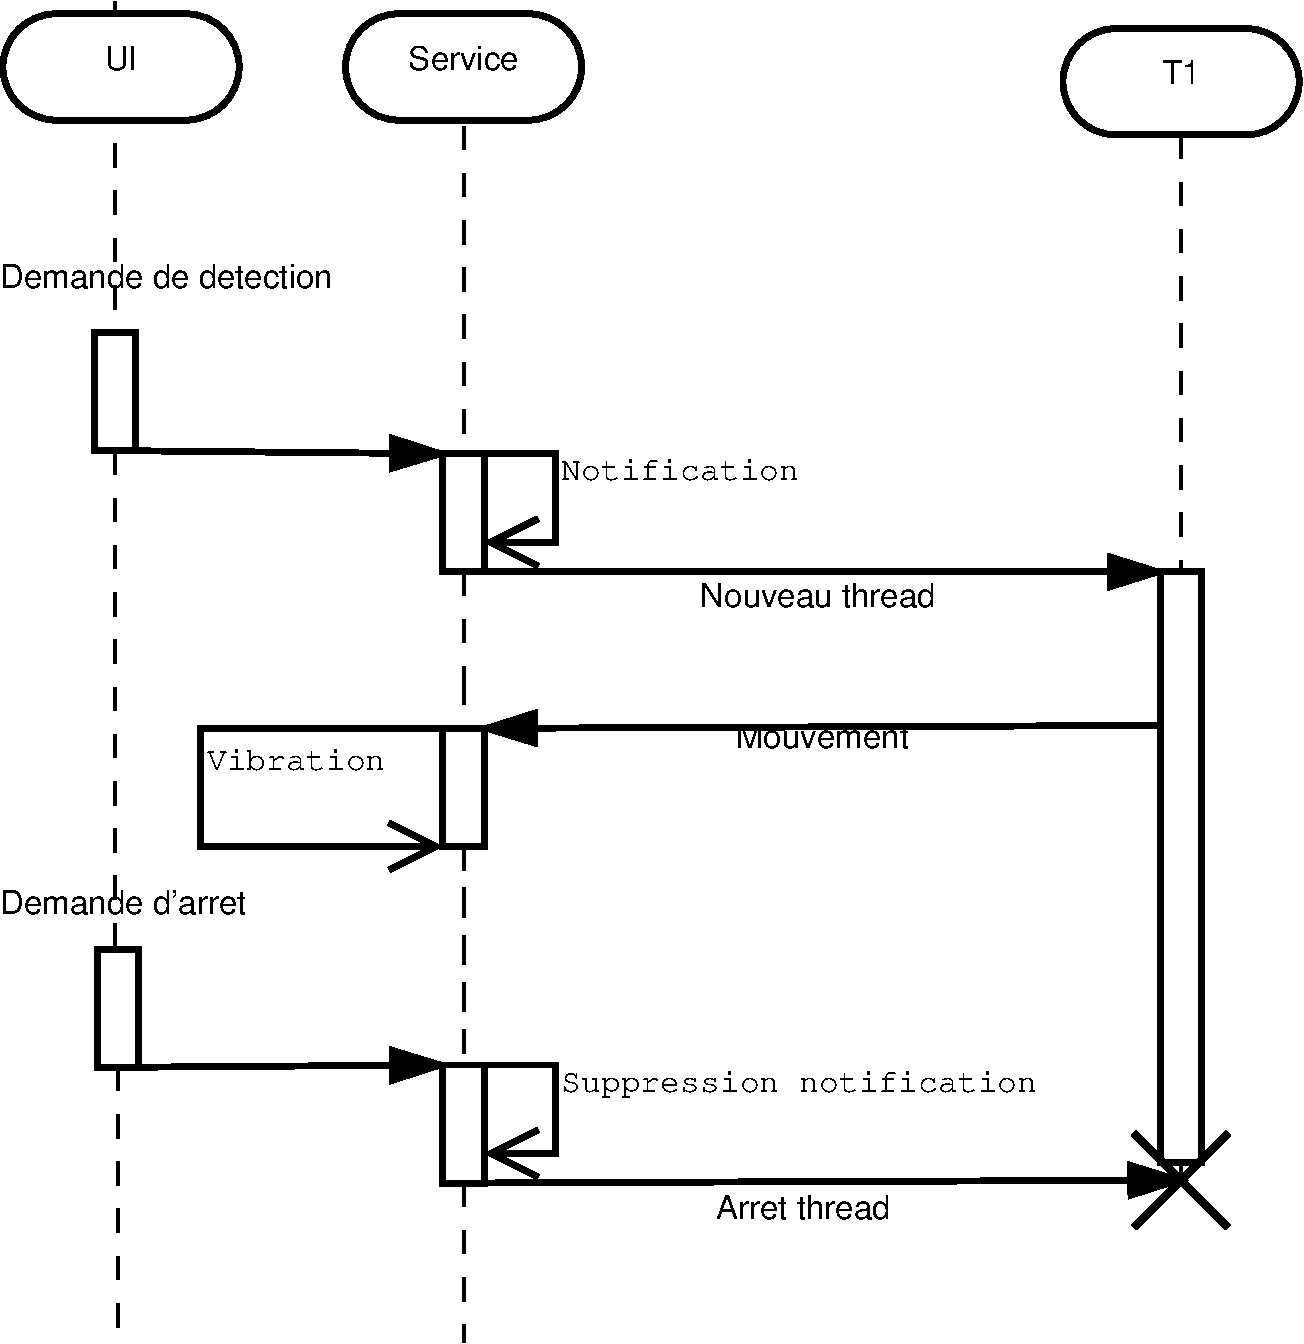
\includegraphics[scale=0.4]{Images/service.pdf}
  \caption{Service Sequence Diagramm}
\end{figure}  
\indent De plus chaque demande de détection de mouvement auprès d'une
caméra créera une notification ``en cours'' dans la barre de notification du téléphone.
Ainsi l'utilisateur pourra accéder facilement et rapidement à la caméra dont il
souhaite surveiller les mouvements.
\begin{figure}[H]
  \label{notifencours}
  \centering
   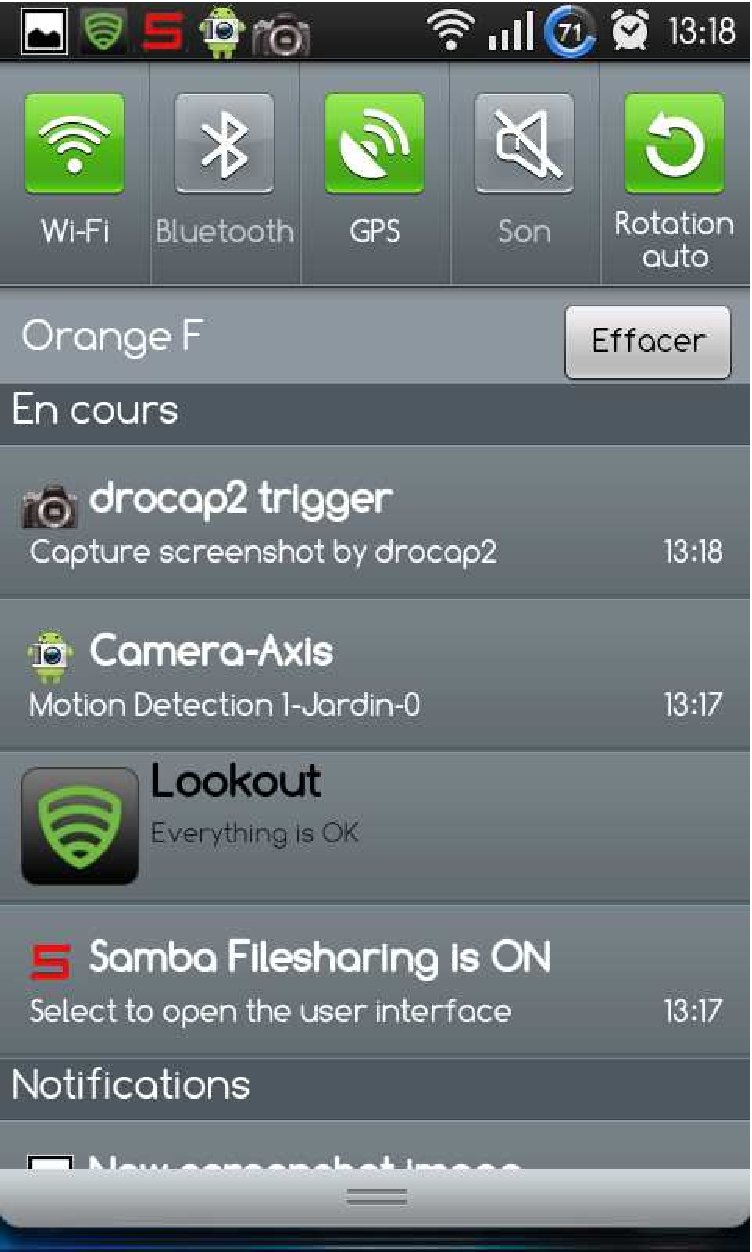
\includegraphics[scale=0.4]{Images/notifencours.pdf}
  \caption{Running Notification}
\end{figure}  
\section{Gestion des préférences}
\subsection{Import / Export}
Cette partie s'intéresse à la sauvegarde de la liste des caméras. En effet si
l'utilisateur décide de desinstaller l'application, ou si il change de
téléphone, nous avons souhaité qu'il ai la possibilité de partager la liste de
ses caméras. Pour ce faire nous avons implémenté deux fonctions pour importer et
exporter cette liste.\newline
La facilitée de modification, et la portabilité du langage \textit{xml} nous a
conduit à formaliser les éléments de cette liste sous forme de différentes
balises imbriquées :
\begin{lstlisting}[language=XML, format=XML]
<?xml version='1.0' encoding='UTF-8' standalone='yes' ?> 
<camList>
   	 <camera> 
   		<id>home</id>
  		<adresse>http://192.168.1.20/</adresse> 
  		<channel>1</channel> 
  	</camera> 
  	<camera> 
   		<id>home ext</id>
  		<adresse>http://82.---.---.---/</adresse> 
  		<channel>1</channel> 
  	</camera> 
</camList>
\end{lstlisting}
Pour des raisons de sécurités évidente, nous n'avons pas souhaité sauvegarder
les noms d'utilisateurs et mots de passe, c'est pourquoi lorsque l'utilisateur
importe ses caméras, il devra tout de même les modifier une à une afin de
remplir les champs en question.\newline
\indent L'écriture et la lecture de se fichier se fait au travers de deux fonctions
:
\begin{lstlisting}
public static void xmlWrite(ArrayList<Camera> camList, String url)
public static ArrayList<Camera> xmlRead(String url)
\end{lstlisting}
La première crée et rempli le fichier en utilisant la classe
\textit{XmlSerializer} à partir des caméras fourni en paramètres.
La seconde lit et alloue une liste de caméras grâce à la classe
\textit{DocumentBuilderFactory} qui nous permet de ``parser'' le fichier afin de
récupérer le contenu de chacune des balises à l'aide de la fonction :
\begin{lstlisting}
doc.getElementsByTagName("camera");
\end{lstlisting}
\indent Nous avons choisis d'exporter les caméras dans une zone mémoire
accessible aux utilisateurs ne disposant pas de téléphone ``rooté''. C'est pourquoi le dossier
de destination par défaut est "/sdcard/com.myapps.camera/". Mais lors de
l'exportation l'utilisateur peut tout de même modifier ce chemin en le modifiant
manuelement lors de l'apparition de l'\textit{AlertDialog}.
\begin{figure}[H]
  \label{export}
  \centering
   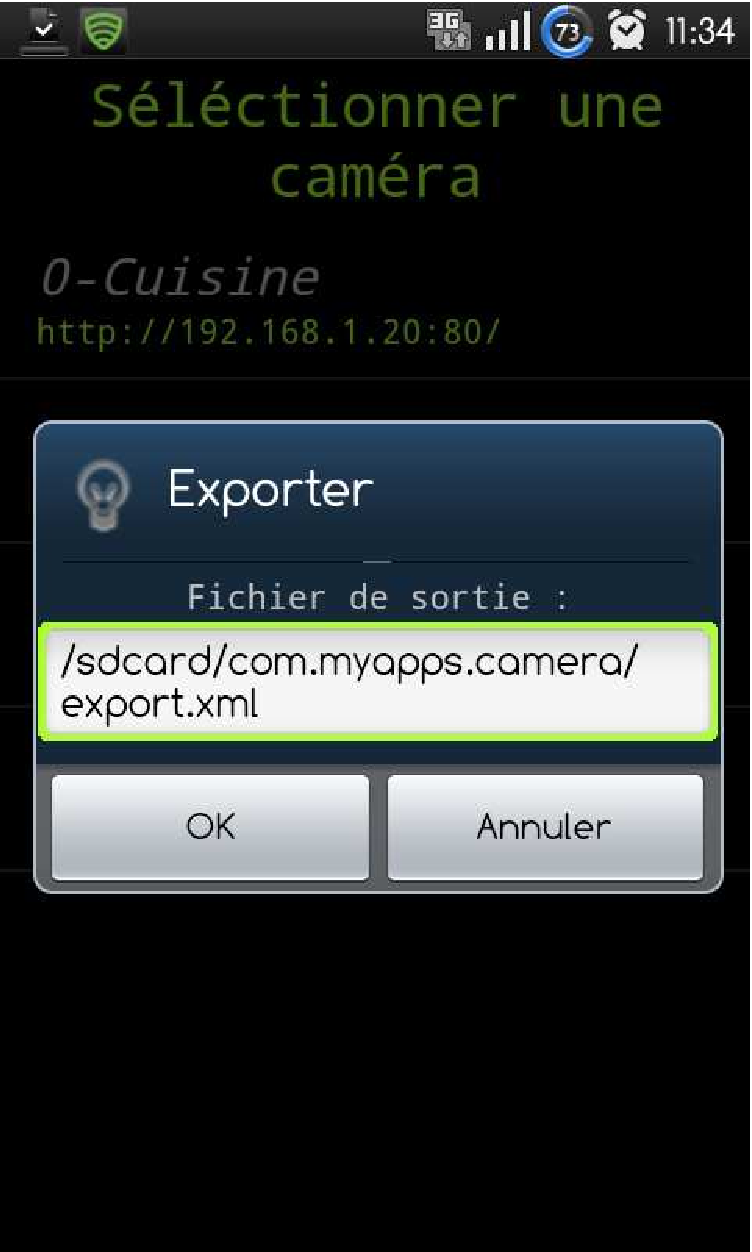
\includegraphics[scale=0.4]{Images/export.pdf}
  \caption{Export Dialog}
\end{figure}  

\subsection{Shared Preferences}
Tout au long de se projet nous avons implémenté un grand nombre de fonction
disposant de paramètres défini par l'utilisateur.
La classe \textit{SharedPreferences} permet de sauvegarder des couples
``donnée/clée'' afin de faire perdurer ces données entre les sessions.\newline
Il est nécessaire d'établir plusieurs étapes pour utiliser cette classe : 
\begin{enumerate}
  \item Implémentation de la vue pour accéder à nos paramètres :
  \begin{lstlisting}[language=XML, format=XML]
  <PreferenceScreen xmlns:android="http://schemas.android.com/apk/res/android"
	xmlns:seekbarattr="http://schemas.android.com/apk/res/com.myapps">

	<PreferenceCategory android:title="Delai">
		<EditTextPreference 
			android:key="limitFPS"
			android:title="Delai FPS" 
			android:numeric="decimal"
			android:summary="Une description"/>
		<EditTextPreference android:key="@string/NotifTO"
			android:numeric="decimal"
			android:title="Delai de Notification Motion Detection"
			android:summary="Une description"/>
	</PreferenceCategory>
	<PreferenceCategory android:title="Autre">
		<CheckBoxPreference 
			android:key="@string/isWelcome"
			android:title="Desactiver l'astuce"
			android:summary="Une description"/>
	</PreferenceCategory>
 </PreferenceScreen> 
  \end{lstlisting}
\item Il faut ensuite créer une classe pour utiliser la vue précedement
défini et initialiser les différents composants :
\begin{lstlisting}
public class MesPreferences extends PreferenceActivity{
@Override
public void onCreate(Bundle savedInstanceState) {
	super.onCreate(savedInstanceState);
	addPreferencesFromResource(R.xml.preferences);
	preferences = PreferenceManager.getDefaultSharedPreferences(this);

/* Show current delay */
	preferenceManagerUtils.setEditTextPreferenceValueFromPreference(this,
		preferences, getString(R.string.TimeOut),
		getString(R.string.defaultTimeOut));
/*	.... */
		}
		}
\end{lstlisting}
\item Il ne reste plus qu'à utiliser le \textit{SharedPreferences} en récupérant
une instance de celui-ci dans l'activité principale : 
\begin{lstlisting}
preferences = PreferenceManager.getDefaultSharedPreferences(this);
/* Print tricky */
if (preferences.getBoolean(getString(R.string.isWelcome), true) == false) {
Dialog_welcome myDialog = new Dialog_welcome(this,R.style.theme_dialog);
myDialog.show();
}
\end{lstlisting}
\end{enumerate}
\indent Nous sommes donc en mesure de régler un nombre illimité de paramètres comme :
\begin{itemize}
  \item Le Delai d'attente entre chaque téléchargement d'image pour le
  \textit{PlayerThread}.
  \item Le temps de non réponse maximum pour un requête \textit{HTTP}.
  \item L'interval entre deux notification lors de la detection de mouvement.
  \item L'activation ou non du pop-up d'astuces au démarrage.
  \item La sensibilité du PTZ réglable a l'aide d'une ``seekBar'' disponible
  en Open Source a l'adresse suivant :\newline
  http://www.codeproject.com/KB/android/seekbar\_preference.aspx
  \item Le seuil de détection de mouvement.
\end{itemize}

\section{Multilangues, Interface  et Partage}
\subsubsection{Multilangues}
Android offre la possibilité à une application d'adapter son langage en fonction
de la langue du téléphone. Nos chaînes de caractères étant déjà regroupées dans
le fichier \textit{res/values/strings.xml}, nous avons décider de traduire
notre application en quatre langues : Allemand, Anglais, Espagnol, Français.\newline
Pour ce faire il suffit de créer 4 fichiers :
\begin{itemize}
\item \textit{res/values-de/strings.xml}
\item \textit{res/values-en/strings.xml}
\item \textit{res/values-es/strings.xml}
\item \textit{res/values-fr/strings.xml}
\end{itemize}
contenant respectivement la traduction des chaînes de caractères en fonction des
langues citées ci-dessus.
\begin{figure}[H]
\centering
  \label{langue}
   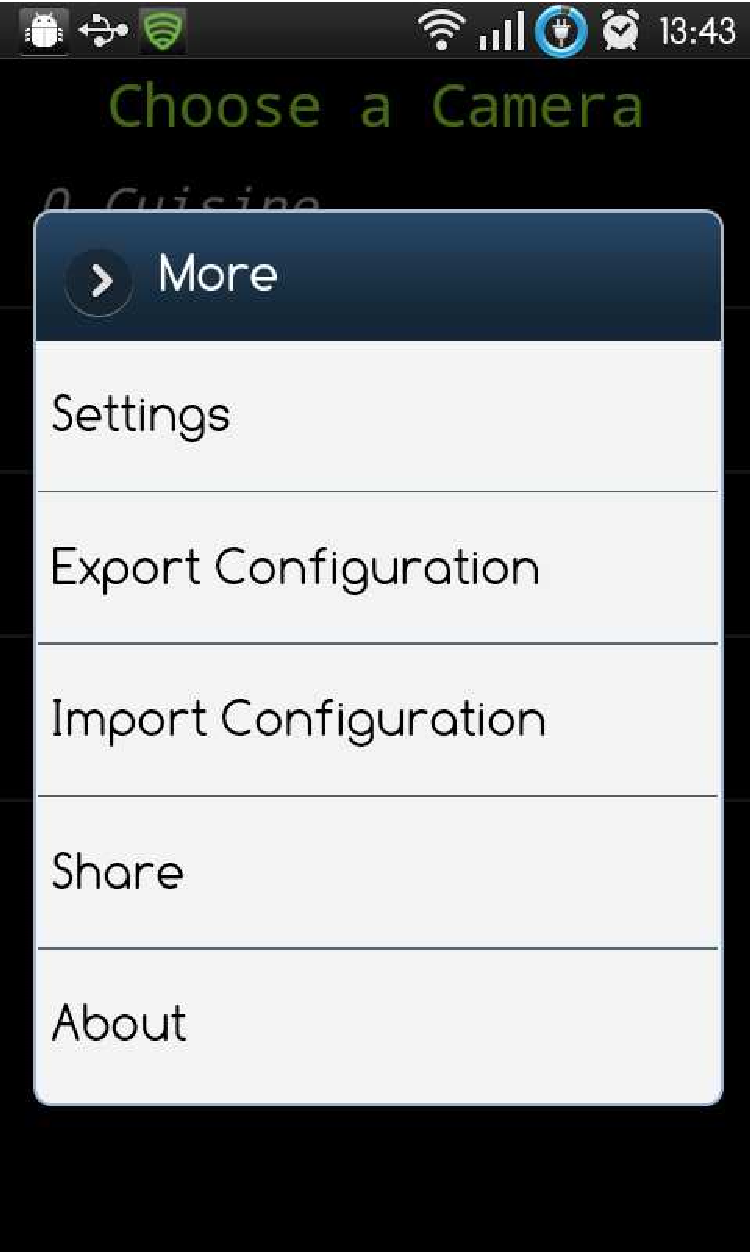
\includegraphics[scale=0.4]{Images/en.pdf}
   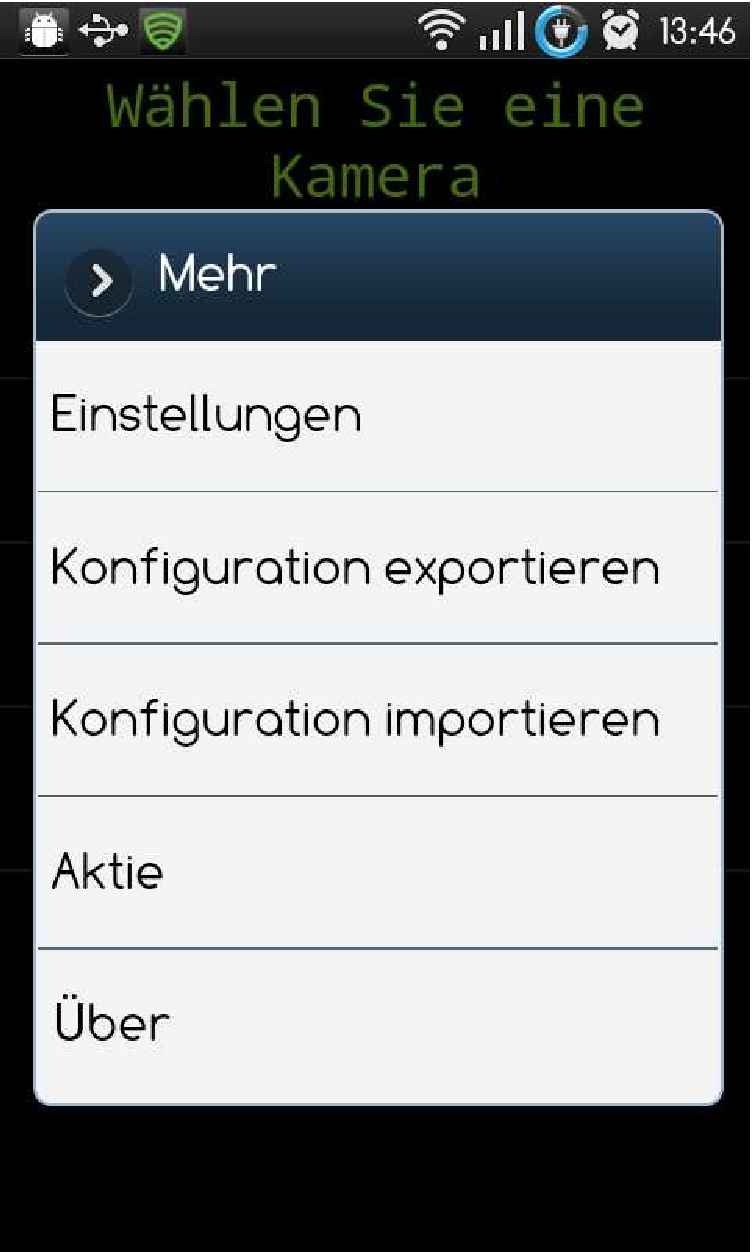
\includegraphics[scale=0.4]{Images/de.pdf}
  \caption{English - Deutsch Translation}
\end{figure}  


\subsubsection{Interface}
Nous avons défini les couleurs, la police, et la taille des différents textes à
l'aide de feuille de styles (équivalent \textit{css} pour Android) dans le
fichier : \textit{res/values/attrs}. L'idée est de surcharger le style par
défaut de chacun des composants graphique afin d'y apporter quelques
modifications (comme la couleur par exemple) créant ainsi notre propre thème
indépendant des thèmes implémentés par les constructeurs (\textit{HTC Sens},
\textit{Samsung TouchWiz}, \textit{Motorola Motoblur}, \ldots).
\begin{lstlisting}[language=XML, format=XML]
<style name="CustomTheme" parent="android:Theme.NoTitleBar">
		<item name="android:colorBackground">
		@color/black
		</item>
		<item name="android:buttonStyle">
		@style/StandardButton
		</item>
		<item name="android:textViewStyle">
		@style/StandardTextView
		</item>
		<item name="android:editTextStyle">
		@style/StandardEditText
		</item>
		<item name="android:listViewStyle">
		@style/StandardListView
		</item>
</style>

<style name="StandardTextView" parent="@android:style/Widget.TextView">
		<item name="android:textColorHint">
		@color/greenyellow
		</item>
		<item name="android:textColor">
		@color/silver
		</item>
		<item name="android:typeface">
		monospace
		</item>
</style>
\end{lstlisting}

\subsubsection{Partage}
Enfin pour finir sur le chapitre concernant l'implémentation, nous avons fourni
à l'utilisateur une fonction permettant le partage de l'application
(respectivement d'une caméra) via un message (resp. un fichier join) pouvant
être diffusé par de nombreuses applications (mail, sms, ``facebook'', \ldots).
Pour ce faire il faut dans un premier temps, définir l'action de
l'intent (dans notre cas nous souhaitons partager des données, nous utilisons donc le flag
\textit{ACTION\_SEND}). Puis il faut spécifier le type des données à partager
(ici il s'agit simplement d'une chaîne de caractères).
Enfin nous pouvons démarrer l'activité choisi lors de l'affichage de
l'\textit{AlertDialog}.
\begin{lstlisting}
    final Intent messIntent = new Intent(Intent.ACTION_SEND);
	    messIntent.setType("text/plain");
	    messIntent.putExtra(Intent.EXTRA_TEXT, getString(R.string.messageShare));
	    startActivity(Intent.createChooser(messIntent, getString(R.string.shareTitle)));
\end{lstlisting}
\begin{figure}[H]
\centering
  \label{partage}
   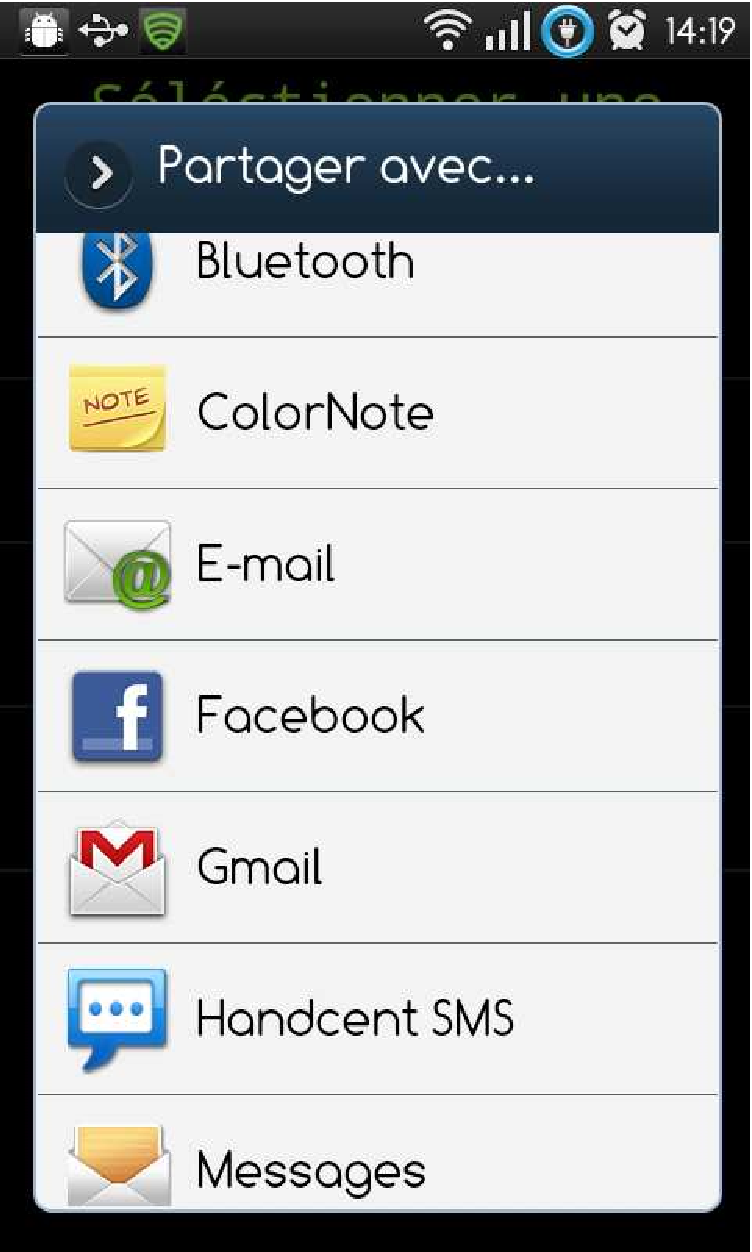
\includegraphics[scale=0.4]{Images/partage.pdf}
  \caption{Share with\ldots}
\end{figure} 

